% Tipo de documento
\documentclass[a4paper,12pt,spanish]{article}

% Configuración de codificación y lenguaje
\usepackage[es-tabla]{babel}
\usepackage[utf8]{inputenc}
\usepackage[T1]{fontenc}    % Buena codificación de fuentes

% Configuración de fuentes y estilo de página
\usepackage{newtxtext,newtxmath}
\usepackage{titlesec}
\usepackage{fancyhdr}
\usepackage{setspace}
\usepackage[margin=1in , headheight=20pt]{geometry}

% Configuración de gráficos, tablas, listas y figuras
\usepackage{caption}
\usepackage{float}
\usepackage{graphicx}
\usepackage{enumitem}
%\usepackage{pdfpages}

% Configuración de matemáticas y unidades
\usepackage{amsmath}
\usepackage{amsfonts}
\usepackage{siunitx}

% Carga del paquete csquotes para manejar citas correctamente
\usepackage{csquotes}
% Carga del paquete biblatex (bibliografía)
\usepackage[backend=biber, style=ieee]{biblatex} 
% Añadir la base de datos de bibliografía
\addbibresource{bibliografia.bib} 

% Configuración de enlaces y referencias
\usepackage[colorlinks=true, urlcolor=blue, linkcolor=black, hidelinks]{hyperref}
\usepackage{lastpage}


%Puedes incluir el código de cualquier LP dentro de un entorno lstlisting utilizando el paquete listings.
\usepackage{listings} 
%Ajusta los colores de tu codigo
\usepackage{xcolor}

% Configuración de interlineado
\setstretch{1.5}

% Configuración de sangría
\parindent=1.27cm

% Configuración de títulos de secciones
\titleformat{\section}{\normalfont\Large\bfseries}{\thesection.}{1em}{}[\titlerule]

% Configuración de Figuras y Tablas
\captionsetup[figure]{labelfont={bf}}
%\captionsetup[table]{labelfont={bf}}

% Configuración de los encabezados y pie de página con fancyhdr
\pagestyle{fancy}
\fancyhf{}
\fancyhead[L]{\textit{\leftmark}}
\fancyhead[R]{\textit{\rightmark}}
\fancyfoot[L]{\textit{Redes Eléctricas III}}
\fancyfoot[C]{\textit{\thepage/\pageref{LastPage}}}
\fancyfoot[R]{\textit{Semestre 2024-1}}
\renewcommand{\footrulewidth}{1pt} % Ancho de la línea divisoria
\renewcommand{\headrulewidth}{1pt} % Establece el ancho de la línea divisoria del encabezado

%Configuración de listings
\lstset{
  language=Python,         % Lenguaje del código
  basicstyle=\ttfamily\small, % Estilo básico de la fuente
  keywordstyle=\color{blue},  % Color de las palabras clave
  commentstyle=\color{gray},  % Color de los comentarios
  stringstyle=\color{red},    % Color de los strings
  breaklines=true,            % Cortar las líneas largas
  frame=single,               % Colocar marco alrededor del código
  captionpos=b                % Posición del título
}
\renewcommand{\lstlistingname}{Código}





\begin{document}
    
    % Portada

\begin{titlepage}
    \begin{center}
        \textsc{\large Universidad Central de Venezuela}\\
        \textsc{\large Facultad de Ingeniería}\\
        \textsc{\large Escuela de Ingeniería Eléctrica}\\
        \textsc{\large Departamento de Electrónica, Computación y Control}\\[7cm]
        
        {\huge \bfseries PRÁCTICA N°3}\\[0.2cm]
        {\Large APLICACIONES NO LINEALES DEL AMPLIFICADOR OPERACIONAL}\\[10cm]
        
        \begin{minipage}{0.4\textwidth}
            \begin{flushleft}
                \emph{Aux. Docente:}\\
                Escobar, Caleb 
            \end{flushleft}
        \end{minipage}
        \begin{minipage}{0.4\textwidth}
            \begin{flushright}
                \emph{Autor:}\\
                Br. Rivero, Axel
            \end{flushright}
        \end{minipage}
        
        \vfill
        
        {\large Caracas, \today} %Fecha actual del documento
        
    \end{center}
\end{titlepage}

    
    \tableofcontents

\newpage
    
    \section{Introducción}

    Las líneas de transmisión eléctricas juegan un papel fundamental en la infraestructura energética moderna, permitiendo la transferencia eficiente de energía desde los centros de generación hasta los puntos de consumo. No obstante, el diseño y la operación de estas líneas presentan una serie de desafíos técnicos que deben ser abordados para optimizar su rendimiento y minimizar las pérdidas de energía. Entre los principales problemas se encuentran las diversas pérdidas de energía que ocurren durante la transmisión, lo que puede reducir la cantidad de energía útil que llega al destino.

    Existen varios tipos de pérdidas en las líneas de transmisión, entre las cuales se destacan las pérdidas resistivas, las pérdidas por radiación, las pérdidas por calentamiento del dieléctrico y las pérdidas por efecto corona. Las pérdidas resistivas, ocurren debido a la resistencia inherente de los materiales conductores y están directamente relacionadas con la longitud de la línea y la corriente que fluye a través de ella. Por otro lado, las pérdidas por radiación y calentamiento del dieléctrico son más prominentes a frecuencias más altas y pueden reducirse mediante el uso de materiales adecuados y técnicas de blindaje. El efecto corona, que ocurre principalmente en líneas de alta tensión, genera pérdidas significativas de energía debido a la ionización del aire alrededor de los conductores.
    
    Este trabajo tiene como objetivo analizar las pérdidas resistivas en los conductores más utilizados en líneas de transmisión: cobre, aluminio y oro. Para ello, se ha implementado una simulación en Python, donde se modelan los efectos de la resistividad, el diámetro del conductor y la corriente sobre las pérdidas de energía. Los resultados obtenidos permitirán proponer soluciones viables para mejorar la eficiencia de las líneas de transmisión, enfocándose en la reducción de las pérdidas de potencia.
    
    Además, se evaluarán métodos para medir y mitigar las pérdidas mencionadas, brindando una visión más completa de las diferentes estrategias de optimización disponibles. Finalmente, se presentarán propuestas de diseño que permitan aumentar la eficiencia de las líneas de transmisión, siempre considerando la viabilidad técnica y económica de cada opción.




\newpage

    \section{Planteamiento del problema}

    Las líneas de transmisión son esenciales en la distribución de energía eléctrica desde los generadores hasta los consumidores. Sin embargo, durante este proceso, se producen diversas pérdidas que afectan la eficiencia del sistema de transmisión. Estas pérdidas no solo representan un costo económico significativo, sino que también impactan la estabilidad y confiabilidad del suministro eléctrico. Es crucial entender y mitigar estas pérdidas para mejorar la eficiencia energética y reducir los costos operativos.
    
    En el ámbito de la transmisión de energía, se identifican varios tipos de pérdidas que ocurren debido a diferentes factores:

    \begin{enumerate}
        \item Pérdida en el conductor.

        \item Pérdida por calentamiento del dieléctrico.

        \item Pérdida por radiación.

        \item Pérdida por acoplamiento.

        \item Efecto corona.
    \end{enumerate}

    \subsection{Objetivo}
    
        El objetivo de este estudio es investigar y analizar los procedimientos para medir cada uno de los tipos de pérdidas mencionados en las líneas de transmisión de energía. Además, se diseñará un montaje práctico en un laboratorio para medir uno de estos tipos de pérdidas, proporcionando así una metodología clara y precisa para su evaluación.

    \subsection{Preguntas de investigación}
    
        \begin{itemize}
            \item ¿Cuáles son los procedimientos más efectivos para medir la pérdida en el conductor en las líneas de transmisión?
            \item ¿Cómo se pueden cuantificar las pérdidas por calentamiento del dieléctrico?    
            \item ¿Qué métodos se utilizan para medir la pérdida por radiación en diferentes condiciones de transmisión?    
            \item ¿Qué técnicas existen para evaluar las pérdidas por acoplamiento entre líneas de transmisión?    
            \item ¿Cómo se puede medir y mitigar el efecto corona en las líneas de transmisión?
        \end{itemize}

    \subsection{Importancia}

        Este estudio es crucial para mejorar la eficiencia de los sistemas de transmisión de energía eléctrica. Al identificar y cuantificar adecuadamente las diversas pérdidas, se pueden desarrollar estrategias más efectivas para mitigarlas.





\newpage
    
    %Marco Teórico
\section{Marco Teórico}
Aproximadamente en el año 1947 se creó el primer transistor y hoy en día se ha convertido en uno de los componentes más útiles y novedosos que podemos encontrar para diversas aplicaciones.

No olvidemos que los transistores iniciaron el camino para la creación de los microprocesadores, los circuitos integrados y las memorias de los computadores.

En la actualidad, la importancia de los transistores en la industria es clave, ya que ofrecen un tipo de tecnología que permite el desarrollo de dispositivos pequeños y muy potentes. Especialmente en aquellas industrias relacionadas con las telecomunicaciones y equipos médicos, entre otras.

\subsection{¿Qué es un transistor BJT?}

\begin{wrapfigure}{r}{0.35\textwidth}
    \centering
    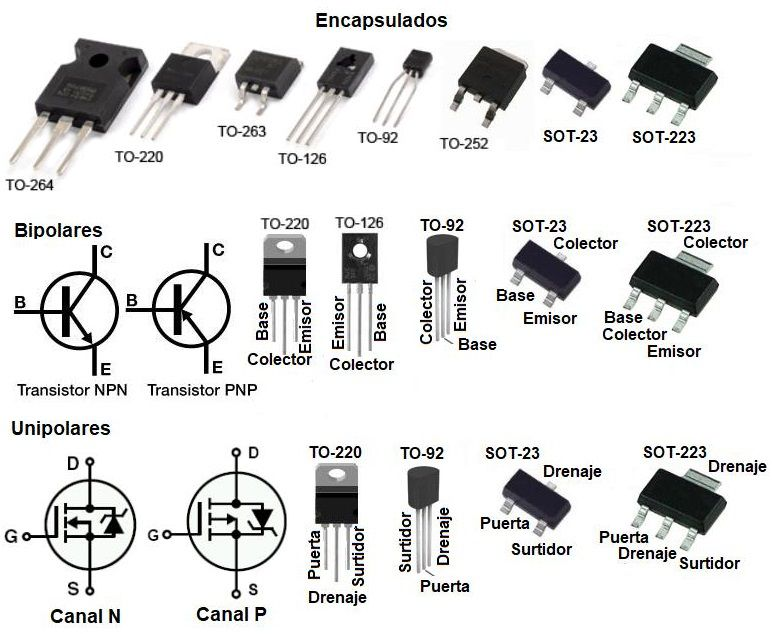
\includegraphics[width=0.35\textwidth]{Imagenes/transistores.jpg}
    \caption{Tipos de transistores}
    \label{fig:transistores}
\end{wrapfigure}

El transistor o BJT es un componente eléctrico semi-conductor que puede ser utilizado para el control adecuado del flujo de corriente eléctrica.


En este caso, una pequeña cantidad de corriente en el conductor base, puede controlar una mayor cantidad de corriente entre el colector y el emisor.

Es por ello que los transistores son muy utilizados en la actualidad para amplificar una señal algo débil (un oscilador o un interruptor, por ejemplo).

En resumen, un transistor puede modificar una señal eléctrica de salida en respuesta a una de entrada, funcionando de esta forma como conmutador, amplificador, rectificador u oscilador.

Entre las características más destacadas de un transistor tenemos:
\begin{itemize}
    \item Es un dispositivo electrónico semiconductor.
    \item Permite el paso de una señal (salida) en respuesta a otra (entrada).
    \item Suelen estar fabricados de cristal de silicio.
    \item Los transistores son sellados herméticamente.
    \item Presentan una carcasa de plástico o una cubierta metálica con tres terminales.
    \item Se puede configurar como amplificador, conmutador, oscilador, o rectificador.
\end{itemize}

\subsubsection{¿Para qué sirven?}

Como ya hemos indicado anteriormente, los transistores son un tipo de dispositivo electrónico que pueden controlar o modificar el flujo de electricidad, siendo ideales para alimentar otros dispositivos pequeños y potentes.

Estos pequeños componentes se elaboran mayormente de silicio y se utilizan en diversos tipos de aparatos electrónicos: teléfonos móviles, tabletas industriales, computadores y robots en las industrias.

Por lo tanto, los transistores tienen diversas aplicaciones en la electrónica y en muchas otras industrias, revolucionado la forma de interactuar entre la tecnología y las actividades cotidianas.
Sin duda, los transistores son un componente muy importante para la industria moderna, ya que permiten circuitos más pequeños y eficientes, y también se pueden usar para diseñar dispositivos digitales de última tecnología.
Adicionalmente, no olvidemos que los transistores pueden ser de tipo “activados o no activados”, y básicamente se diferencian en la forma en que funciona cada uno de ellos.

\subsubsection{¿Cómo funciona un transistor?}
El objetivo principal de un transistor es permitir la transferencia adecuada de energía eléctrica entre las diferentes partes de un circuito eléctrico.

Por lo tanto, los transistores controlan o cambian el flujo de electricidad entre dos puntos, y vienen en muchas formas y tamaños.

Los transistores se utilizan en todo tipo de aparatos electrónicos: desde teléfonos móviles y tabletas, hasta computadores y robots en las industrias.

En términos generales, estos trabajan sobre un flujo de corriente, funcionando como amplificadores al recibir una señal débil y generando una señal más fuerte, o como interruptores al recibir una señal y cortar su paso.

Normalmente, esto ocurre dependiendo de las posiciones que ocupe un transistor en un determinado instante:
\begin{itemize}
    \item \textbf{Posición activa}: aquí se permite el paso de un nivel de corriente variable
    \item \textbf{En corte}: en esta posición no se deja pasar la corriente eléctrica
    \item \textbf{En saturación}: aquí se deja pasar toda la corriente eléctrica (corriente máxima)
\end{itemize}



En cuanto a las partes de un transistor, este se compone de 3 elementos clave: hablamos de la base, colector y emisor.

En ese caso, la base intercede entre el emisor por donde entra la corriente y el colector por donde sale el caudal de corriente.  Es por ello que, si la base de un transistor no recibe corriente eléctrica, este se ubicará en posición de corte. En cambio, si el transistor recibe un flujo de corriente intermedia, la base puede abrir el flujo en una determinada cantidad.

Y, por último, si la base recibe un gran flujo de corriente eléctrica, entonces se abrirá al máximo para pasar el total de la corriente modulada.

Ahora, teniendo un conocimiento previo de lo que es un transistor, se puede saber un poco más sobre como de ese pequeño dispositivo, se puede realizar un análisis detallado de sus configuraciones mas importantes y de ellos crear las etapas que se estudiarán mas adelante.

\subsection{Corrientes del transistor BJT}

Se debe tener en cuenta lo siguiente con las corrientes de los transistores:


\subsubsection{Corriente de colector}
\begin{equation}
    I_C=\beta I_B
    \label{eqn:ic}
\end{equation}
\subsubsection{Corriente de base}
\begin{equation}
    I_B=\dfrac{I_C}{\beta }
    \label{eqn:ib}
\end{equation}
\subsubsection{Corriente de emisor}
\begin{align}
    I_E & =I_B+I_C \label{eqn:ie}                                                                       \\[0.2cm]
    I_E & =\dfrac{I_c}{\beta}+I_C=(\dfrac{1}{\beta}+1)I_C =\dfrac{1+\beta}{\beta}I_C  \label{eqn:ie_ic} \\[0.2cm]
    I_E & = I_B+\beta I_B = I_B(1+\beta) \label{eqn:ie_ib}
\end{align}
\subsection{Configuraciones básicas del BJT}

Los transistores son uno de los componentes más utilizados dentro de la electrónica ya que tienen diferentes configuraciones y polarizaciones, y dependiendo de las variaciones estos funcionan de forma diferente. Cuando se quiere utilizar un transistor como interruptor digital (regiones de corte y saturación) la tarea es fácil ya que el circuito eléctrico es bastante sencillo. En caso de que se utilicé un transistor NPN el emisor se coloca a tierra, el colector a voltaje y la base actúa como interruptor, o si bien se utiliza un transistor PNP se invierten las terminales, el colector a tierra y al emisor se le pone voltaje.

\begin{figure}[H]
    \centering
    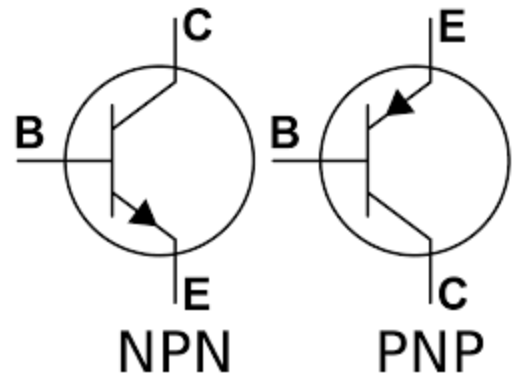
\includegraphics[width=5cm]{Imagenes/simbolo_bjt.png}
    \caption{Símbolo esquemático para cada unos de los transistores BJT}
    \label{fig:simbologia}
\end{figure}

\subsubsection{Emisor Común (EC)}

Esta configuración se utiliza para amplificadores de corriente y voltaje a bajas frecuencias, debido a que tiene una alta ganancia en las dos variables. Una de sus características no tan favorables es que el voltaje de la señal queda invertido en su salida (la corriente no se invierte), es decir las señales quedan como si fueran un espejo. Una forma sencilla de identificar esta configuración es por que la señal de entrada esta en la base y la de salida en el colector. Esta configuración se puede utilizar con todos los tipos de polarizaciones.

\subsubsection{Colector Común (CC)}

Se utiliza para señales con baja potencia y las transforma en el mismo tipo de señal pero con una mayor potencia. Esto se logra por que tiene una alta ganancia de corriente y el voltaje lo transfiere igual ya que no tiene ganancia de voltaje. Otra característica es que en la salida se invierte la corriente. El colector común se utiliza principalmente cuando se requiere poner varios amplificadores conectados en serie debido a que en su entrada tiene mucha impedancia y en su salida disminuye.


\subsubsection{Base Común (BC)} Existen dos formas sencillas de identificar si un transistor esta configurado en base común y estas son; por que el símbolo del transistor se utiliza acostado o porque la entrada es a través del emisor y la salida se encuentra en el colector. A pesar de que esta configuración no tiene una ganancia de corriente se utiliza por que el ancho de banda es más grande que las demás configuraciones y permite trabajar con señales VHF (very high frequency) y UHF (ultra high frequency).


\begin{figure}[H]
    \centering
    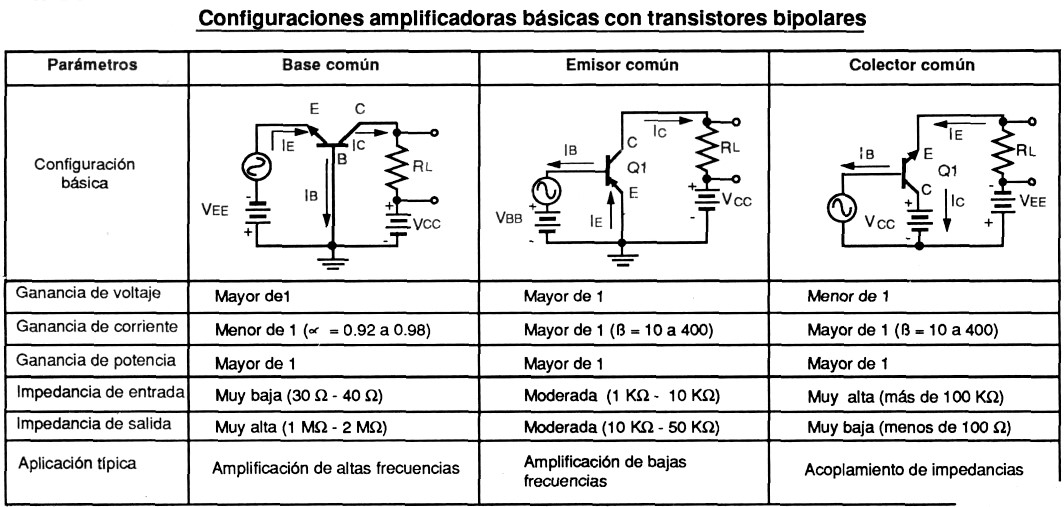
\includegraphics[width=\textwidth]{Imagenes/Configuraciones BJT basicas.jpg}
    \caption{Resumen de configuraciones de los transistores}
    \label{fig:configuraciones}
\end{figure}

Para el cálculo del modelo pi las ecuaciones son distintas
dependiendo su configuración (EC, CC o BC)

\subsection{Polarizaciones de un transistor BJT}

En simples palabras las polarizaciones son circuitos que se utilizan para hacer funcionar a los transistores como amplificadores, en estos circuitos basan su funcionamiento en las configuraciones anteriores, ya que podemos utilizar una de emisor común y utilizar cualquiera de las polarizaciones disponibles todo depende de la aplicación que se le dé al transistor.

\subsubsection{Polarización fija o de base}
Esta polarización solo se puede utilizar con la configuración de emisor común y consiste en colocar una resistencia en la base y una en el colector, mientras que el emisor se conecta a tierra, Al ser una configuración demasiado sencilla tenemos una gran desventaja y es que la señal esta muy expuesta a variaciones dependiendo de los cambios de temperatura que tenga el transistor. Regularmente se utiliza para señales de poca importancia que no importa que se distorsionen.

\subsubsection{Polarización por retroalimentación del emisor o estabilizado en el emisor}
En este tipo prácticamente se le agrega una resistencia en el emisor que hace sea un poco más estable, pero no lo suficiente como para utilizarlo en señales de mucha importancia.

\subsubsection{Polarización por retroalimentación de colector}
Prácticamente se utiliza para regular los cambios de corriente o de voltaje en la fuente de alimentación, ya que si por alguna razón existe una variación, la resistencia que retroalimenta la base actúa para evitar un cambio brusco en la salida del transistor.

\subsubsection{Polarización universal o divisor de voltaje}
Es la más utilizada ya que es la más estable, debido a sus retroalimentaciones. Y si por cualquier razón el transistor se calienta o existen una variación de la corriente la resistencias de retroalimentación actúan para regular la corriente que llega a la base y así poder estabilizar todo el sistema.

\begin{figure}[H]
    \centering
    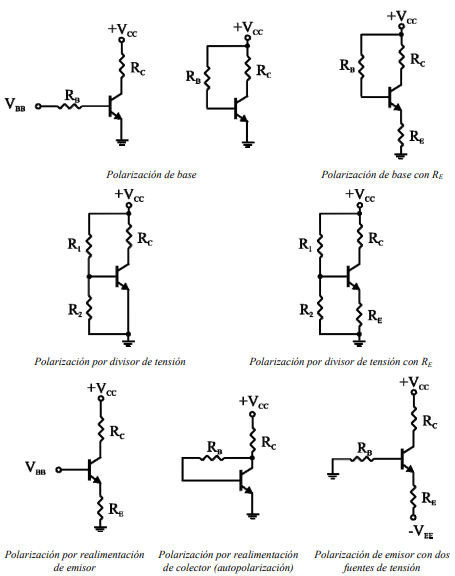
\includegraphics[width=\textwidth]{Imagenes/polarizacion.png}
    \caption{Diferentes circuitos empleados en la polarización de un transistor}
    \label{fig:polarizacion}
\end{figure}

\begin{figure}[H]
    \centering
    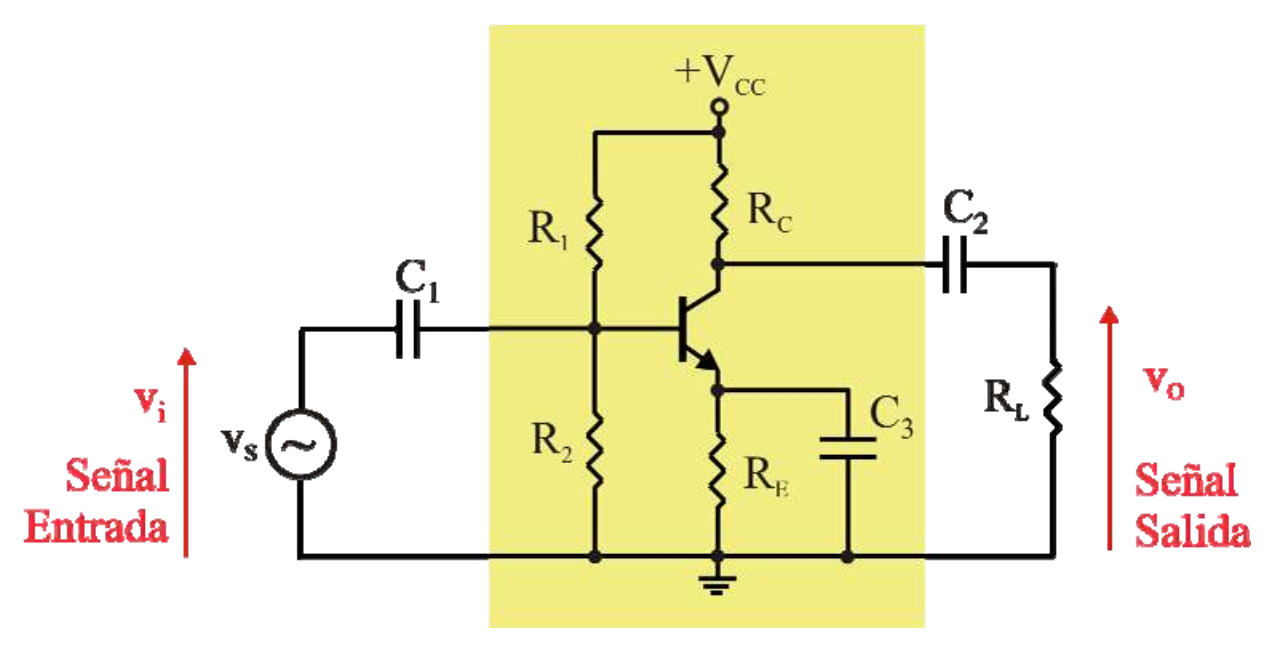
\includegraphics[width=\textwidth]{Imagenes/bjt_ec.png}
    \caption{Circuito amplificador de tensión con BJT en EC}
    \label{fig:ec}
\end{figure}

\subsection{Condensadores de acople y desacople}
En el circuito de la figura \ref{fig:ec} se muestra un circuito típico de un amplificador de tensión con un transistor BJT en emisor común polarizado en la zona activa.
Con él se trata de amplificar una tensión cualquiera vi y aplicarla, una vez amplificada, a una carga que simbolizamos por la resistencia RL. La zona sombreada
resalta el amplificador, que en este caso, lo constituye un transistor BJT en la configuración emisor común. El cual, convenientemente polarizado en la zona activa, es
capaz de comportarse como un amplificador de tensión como ya se mencionó anteriormente.

Los condensadores $C_1$ y $C_2$ que aparecen se denominan condensadores de acoplo y sirven para bloquear la componente continua. En concreto $C_1$ sirve para acoplar la tensión que queremos amplificar al amplificador propiamente dicho, eliminando la posible componente continua que esta tensión pudiera tener. Si no bloqueásemos esta continua se sumaría a las corrientes de polarización del transistor modificando el punto
de funcionamiento del mismo. Por otra parte, el condensador $C_2$ nos permite acoplar la señal amplificada a la carga, eliminando la componente continua (la correspondiente al punto de polarización del transistor) de forma que a la carga llegue únicamente la componente alterna.

El condensador $C_3$ es un condensador de desacoplo, su misión es la de proporcionar un camino a tierra a la componente alterna. En el capítulo anterior se
analizó el efecto de la resistencia $R_E$ desde el punto de vista de su efecto en la estabilización del punto de polarización. Sin embargo, en este capítulo veremos como
desde el punto de vista de la amplificación, esta resistencia hace disminuir la ganancia del amplificador. Al añadir el condensador de desacoplo conseguimos que la continua pase por $R_E$ mientras que la alterna pasaría por el condensador $C_3$ consiguiendo que no
afecte a la amplificación.

\subsection{Principio de superposición}
En este informe vamos a abordar el análisis de este tipo de circuitos amplificadores. Para ello aplicaremos el principio de superposición. En cada punto o rama calcularemos las tensiones y corrientes de continua y de alterna por separado, de forma que al final las tensiones y corrientes finales serán la suma de las calculadas en
cada parte.

Para ello vamos a suponer que el valor de la capacidad de los condensadores, así como la frecuencia de las señales que tenemos es tal que la impedancia que presentan
los condensadores es lo suficientemente pequeña para considerarla nula. Mientras que en continua, estos condensadores presentarán una impedancia infinita. Es decir, consideraremos que en continua los condensadores se comportan como circuitos abiertos (impedancia $\infty$) mientras que en alterna equivaldrán a cortocircuitos (impedancia $0$)

\begin{equation}
    |x_c|=\dfrac{1}{\omega \cdot C}=\dfrac{1}{2\pi f \cdot C}
    \label{eqn:capacitores}
\end{equation}

\begin{figure}[H]
    \centering
    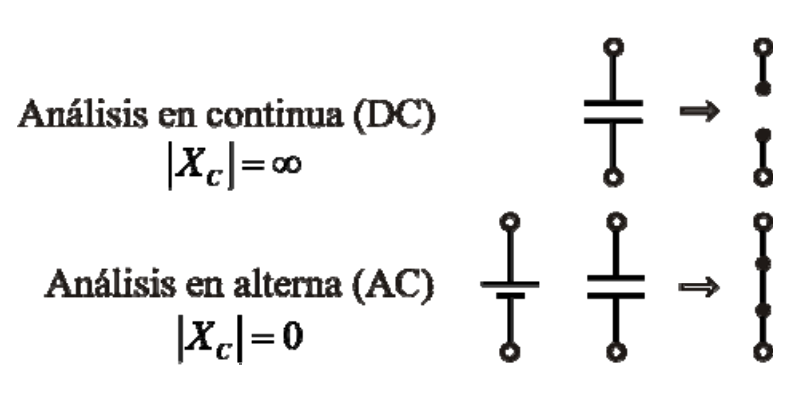
\includegraphics[width=8cm]{Imagenes/analisis_condensadores.png}
    \caption{Consideraciones para aplicar el principio de superposición.}
    \label{fig:consideraciones}
\end{figure}

Aplicando estas consideraciones obtendremos los circuitos equivalentes en DC y en AC que tendremos que resolver separadamente.

Si en el circuito amplificador de la figura \ref{fig:ec} aplicamos la condición de que los condensadores se comportan como circuitos abiertos, obtenemos el circuito equivalente en continua (figura \ref{fig:universal}). Podemos ver como este circuito es, precisamente, el circuito de polarización del transistor cuyo estudio ya se abordó en el punto anterior y de cuya
resolución obtendríamos las tensiones y corrientes de continua presentes en el circuito.

\begin{figure}[H]
    \centering
    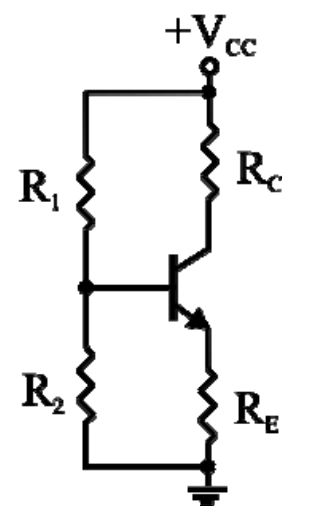
\includegraphics[width=3cm]{Imagenes/universal.png}
    \caption{Circuito equivalente en DC de la figura \ref{fig:ec}}
    \label{fig:universal}
\end{figure}

\subsection{Punto de operación Q}

El punto de operación, es un punto fijo sobre las curvas características, se le conoce también como punto quiesciente (abreviado punto Q). Por definición, quiescente significa quieto, inmóvil, inactivo.

En general, lo importante es calcular los valores de voltajes y corrientes del transistor para una polarización dada. Por tal motivo, se agregara la letra Q a cada
una de los términos que se desean obtener y que son: la corriente de base $I_{BQ}$; la corriente de colector $I_{CQ}$; la corriente de emisor $I_{EQ}$; el voltaje base-emisor $V_{BEQ}$ y el voltaje colector-emisor $V_{CEQ}$. En la mayoría de los casos, la corriente de base $I_{BQ}$ es la primera cantidad que se determina junto con el voltaje base emisor $V_{BEQ}$, una vez que $I_{BQ}$ se conoce, las relaciones de las ecuaciones de malla pueden aplicarse para encontrar las restantes variables como la corriente de colector $I_{CQ}$, etc. Las similitudes en los análisis serán inmediatamente obvias y
las ecuaciones son tan similares para diversas configuraciones que una ecuación
de malla puede derivarse de otra quitando o agregando términos.

\subsection{\texorpdfstring{Modelo $\pi$}{Modelo pi}} %Esta sintaxis es para que no tengo errores al ser referenciado por el entorno hyperref.


\subsubsection{Modelo Pi-híbrido básico del transistor BJT}
Antes de pasar a estudiar el modelo Pi híbrido del transistor voy a compartir un diagrama con la nomenclatura asociada al transistor BJT, con las terminales y las corrientes y voltajes de interés en este dispositivo.

\begin{figure}[H]
    \centering
    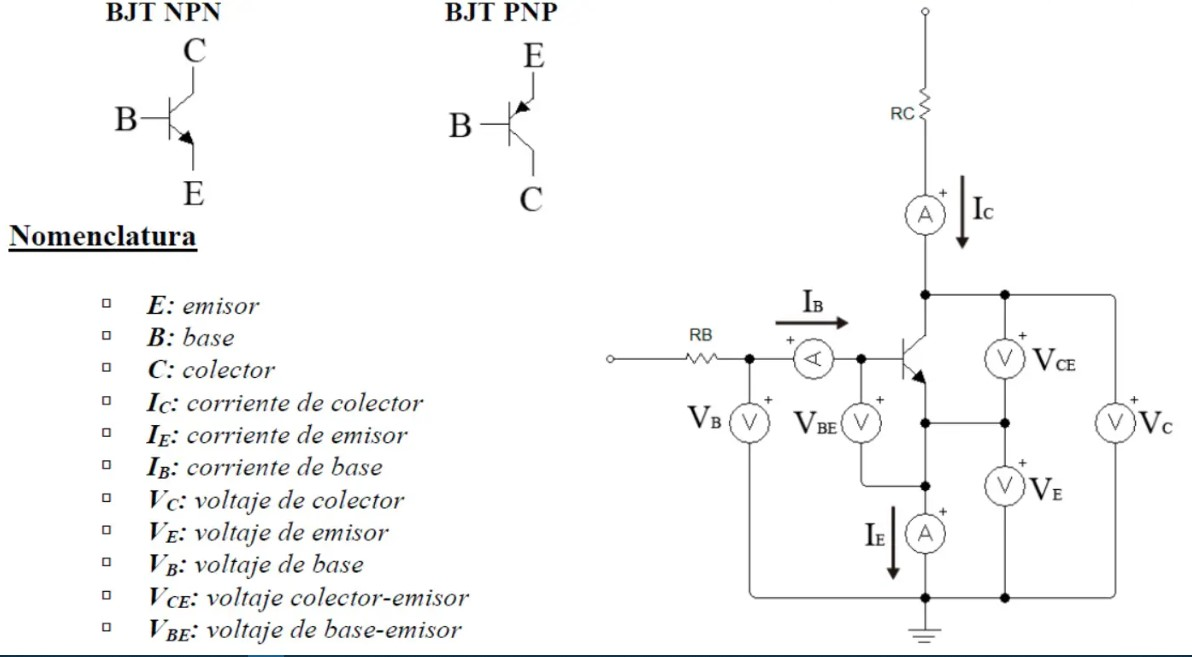
\includegraphics[width=\textwidth]{Imagenes/bjt.jpg}
    \caption{Nomenclatura del BJT}
    \label{fig:bjt}
\end{figure}

Es importante conocer estos términos y como calcularlos, pues de ello dependerá el Modelo Pi. El modelo Pi-híbrido es un modelo de circuito eléctrico que te permite remplazar un transistor en un circuito electrónico por un circuito basado en una fuente dependiente, que facilita el análisis del comportamiento del transistor en condiciones cuando se aplica una señal de frecuencia variable en la entrada del transistor. Básicamente es una convención que permite analizar circuitos con transistores en condiciones de corriente alterna.

Para usar el modelo Pi será necesario remplazar el transistor por un modelo equivalente, el cual se muestra a continuación:

\begin{figure}[H]
    \centering
    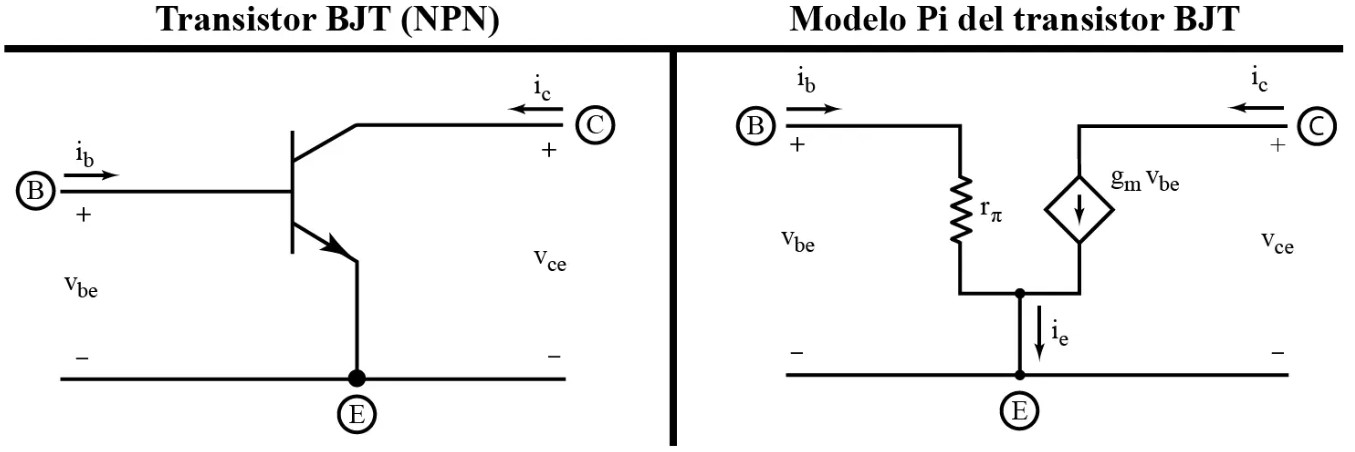
\includegraphics[width=10cm]{Imagenes/modelopi.jpg}
    \caption{Modelo $\pi$}
    \label{fig:modelo_pi}
\end{figure}

Para utilizar el modelo Pi, hace falta calcular dos parámetros: la resistencia $\pi$ y la transconductancia \textbf{$g_m$}. Estos parámetros se calculan utilizando las siguientes ecuaciones:

\begin{gather}
    \mathbf{r_{\pi}} = \dfrac{V_{be}}{i_b} = \dfrac{V_T}{I_{BQ}} = \beta \dfrac{V_T}{I_{CQ}} \label{eqn:rpi}
\end{gather}

\begin{gather}
    \mathbf{g_m}= \dfrac{I_{CQ}}{V_T} \label{eqn:gm}
\end{gather}

En estas ecuaciones la $\beta$ es la ganancia del transistor, la cual es un dato del propio transistor. Este dato casi siempre lo proporciona el enunciado del problema que estemos trabajando. $v_T$ es el voltaje térmico, el cual es aproximadamente 0.026 voltios a la temperatura ambiente (27 ºC). Los sub índices que contienen Q hacen referencia a condiciones de carga.

\subsubsection{Voltaje térmico}

El voltaje térmico ($V_T$) de un transistor bipolar de juntura (BJT) es un parámetro importante que se refiere a la tensión necesaria para mantener una corriente específica en el transistor. Este parámetro es fundamental para entender el comportamiento del transistor en diferentes condiciones de temperatura y corriente.

Se define como la tensión necesaria para mantener una corriente específica en el transistor, usualmente medida entre el colector y la base. Este parámetro es importante porque la temperatura del transistor puede afectar su comportamiento, y el voltaje térmico es una medida de cómo se ajusta la tensión para compensar estos cambios.

\begin{itemize}
    \item Efecto de la temperatura

          Cuando la temperatura del transistor aumenta, la corriente de colector también aumenta debido a que la cantidad de portadores minoritarios en el material semiconductor aumenta. Esto se traduce en un aumento en la corriente de colector. El voltaje térmico se ajusta para compensar este aumento, manteniendo constante la corriente de colector.
    \item Importancia en el diseño

          El voltaje térmico es crucial en el diseño de circuitos que utilizan transistores BJT, ya que permite ajustar la tensión para mantener constante la corriente en diferentes condiciones de temperatura. Esto es especialmente importante en aplicaciones que requieren estabilidad y precisión, como en sistemas de control y amplificación.
\end{itemize}

Siguiendo la siguiente ecuación:

\begin{gather}
    V_T=\dfrac{K \, T}{q}
\end{gather}

Donde, \\
$K$: Constante de Boltzmann $= 1.3806 \, x 10^{-23}$. \\
$q$: Carga del electron $= 1.609 \,x 10^{-19}$. \\
$T$: Temperatura ambiente (en Kelvin) $=25^{\circ} C=298.15 Kelvin$

Teniendo todas las condiciones adecuadas, el valor del voltaje térmico es de $V_T=25.865 m\volt$

\subsubsection{Forma expandida del modelo Pi-híbrido}

El modelo Pi-híbrido expandido toma en cuenta algunos efectos que se producen cuando el transistor opera en condiciones de frecuencia variable y altas frecuencias. A continuación se presenta el modelo Pi-híbrido expandido:

\begin{figure}[H]
    \centering
    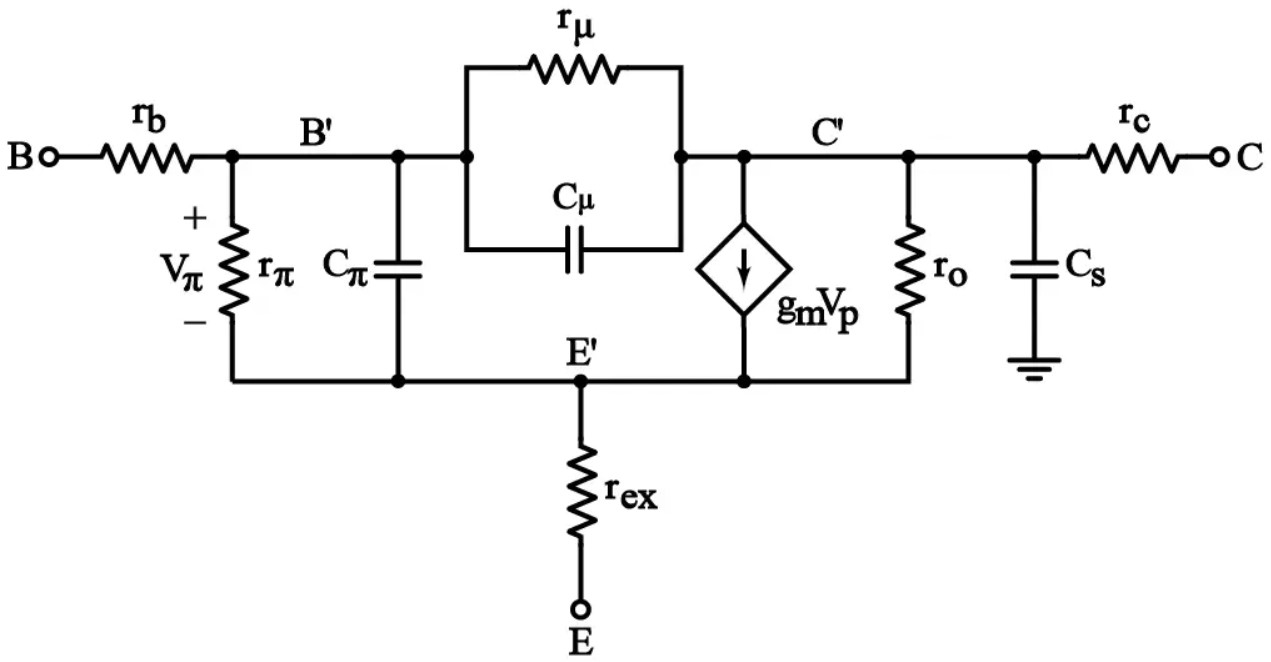
\includegraphics[width=10cm]{Imagenes/modelo pi wh.jpg}
    \caption{Modelo $\pi$ en altas frecuencias}
    \label{fig:modelo_pi_2}
\end{figure}

A continuación procedemos a describir cada uno de los elementos de este modelo:

\begin{itemize}
    \item \textbf{$r_b$, $r_c$, $r_{ex}$:} son resistencias parásitas que se forman en la base, colector y emisor del transistor. Estas resistencias quedan conectadas en serie a las resistencias de base (\textbf{$r_b$}), colector (\textbf{$r_c$}) y emisor (\textbf{$r_{ex}$}). Típicamente poseen valores bajos, entre 1$\Omega$ y 2$\Omega$, por lo cual pueden ser despreciadas.
    \item\textbf{$C_s$:} es la capacitancia del sustrato con el que se construye el transistor. Normalmente posee un valor despreciable. En inglés se conoce como \textbf{junction capacitance of the reverse biased collector–substrate junction}.
    \item\textbf{$C_{\pi}$ y $C_{\mu}$:} son capacitancias asociadas a la juntura del transistor. En inglés se conocen como \textbf{forward-biased junction capacitance o input capacitance} y \textbf{reverse-biased junction capacitance o output capacitance}, respectivamente. Normalmente $C_{\mu}$ es mucho más pequeña que $C_{\pi}$. Sin embargo, por un efecto llamado \textbf{Efecto Miller}, esta capacitancia no puede ser despreciada.

    \item \textbf{$r_\pi$ y $r_{\mu}$:} son resistencias que aparecen en el modelo de corriente alterna. \textbf{$r_{\pi}$} ya la conocemos y sabemos calcularla; \textbf{$r_{\mu}$} es una resistencia con un valor muy alto, típicamente en el orden de los megaohms, por lo cual puede ser despreciada.
\end{itemize}

Algunos de los valores mostrados en el modelo expandido son despreciables por tratarse de resistencias (similar a un circuito abierto) o muy pequeñas (similar a un corto circuito).

\subsubsection{Modelo Pi con efecto Early}

El voltaje Early (denotado por $V_A$) es otro dato del transistor. Es un voltaje que se ubica entre $50$ y $300 V$ y está asociado a la pendiente de las curvas de de polarización del transistor. Este voltaje produce una resistencia denotada por ro que se ubica en la salida del modelo equivalente del transistor, es decir, entre colector y emisor.

\begin{figure}[H]
    \centering
    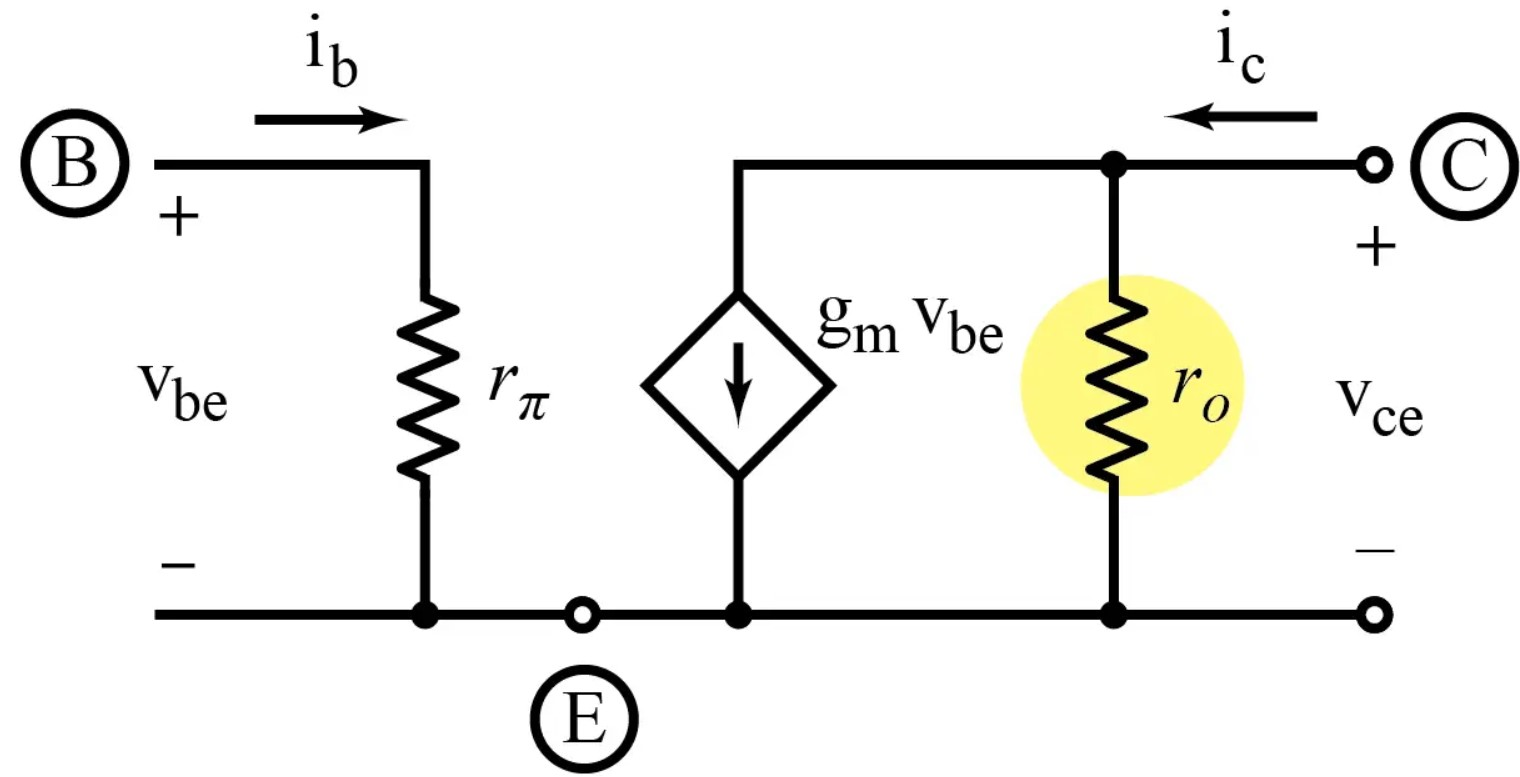
\includegraphics[width=8cm]{Imagenes/modelo_pi3.jpg}
    \caption{Modelo $\pi$ con efecto Early}
    \label{fig:modelo_pi3}
\end{figure}

Para calcular la resistencia $r_o$ se utiliza la siguiente ecuación:

\begin{gather}
    \mathbf{r_o} = \dfrac{V_{A}}{I_{CQ}} \label{eqn:ro}
\end{gather}

Esta resistencia normalmente es de un valor alto, razón por la cual es posible despreciarla. Todo dependerá si se cuenta con un valor de $V_A$, el cual es un dato proporcionado en el enunciado del problema. En otras palabras, es un dato de la hoja de datos del propio transistor.

\subsection{Teorema Miller}

El Teorema de Miller permite redefinir el modelo de corriente alterna del BJT para considerar el efecto de la capacitancia $C_{\mu}$, la cual ya mencionamos en las secciones anteriores de este documento. Sin entrar mucho en detalles, el Teorema de Miller permite hacer lo siguiente:


\begin{figure}[H]
    \centering
    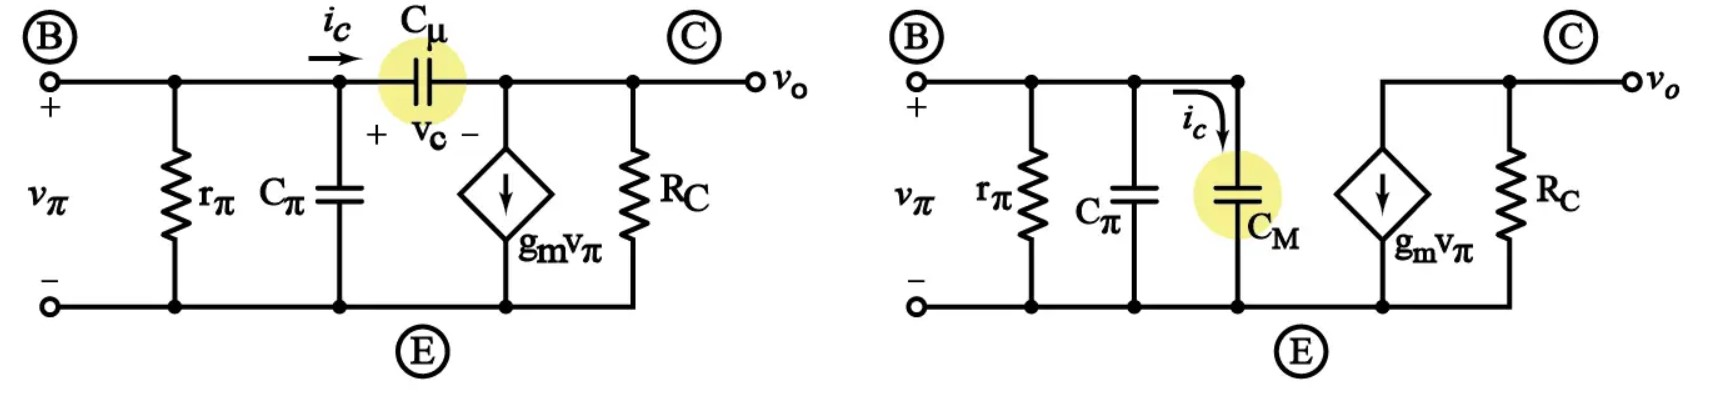
\includegraphics[width=\textwidth]{Imagenes/teorema_miller.jpg}
    \caption{Modelo $\pi$ en altas frecuencias equivalente por el Teorema Miller}
    \label{fig:miller}
\end{figure}

Para hacer la conversión de $C_{\mu}$ a $C_M$ se utiliza la siguiente ecuación:

\begin{equation}
    \mathbf{C_M} =  C_{\pi} + C_{\mu}(1+g_mZ_{out}) = C_{\mu}(1+|A_v|) = \mathbf{C_{eq}} \label{eqn:C_eq}
\end{equation}

En esta ecuación $A_v$ es la ganancia de voltaje del amplificador. Esta ganancia se obtiene al dividir el voltaje de salida entre el voltaje de entrada.

\subsubsection{Resistencia de difusión o intrínseca del emisor ($r_x$)}

$r_x$ en el contexto de transistores bipolares puede referirse a la resistencia de difusión ($r_e$ o resistencia intrínseca del emisor) en el modelo híbrido, no es una nomenclatura estándar comúnmente utilizada en los datasheets de los transistores.

Para calcular la resistencia de difusión se usa la siguiente formula:

\begin{gather}
    r_x=\dfrac{V_T}{I_{E}} \label{eqn:rx}
\end{gather}



\subsection{Ganancia de un amplificador}

Debido a que los amplificadores tienen la capacidad de aumentar la magnitud de una señal de entrada, es útil poder calificar la capacidad de amplificación de un amplificador en términos de una relación salida/entrada. El término técnico para la relación de magnitud salida/entrada de un amplificador es ganancia. Como una relación de unidades iguales (salida de energía/entrada de energía, salida de voltaje/ entrada de voltaje o salida de corriente/entrada de corriente), la ganancia es naturalmente una medición sin unidades.

Matemáticamente, la ganancia está simbolizada por la letra mayúscula “A”.

Las ganancias del amplificador eléctrico se pueden expresar en términos de voltaje, corriente y/o potencia tanto en CA como en CC.

Un resumen de las definiciones de ganancia es el siguiente:

El símbolo “delta” en forma de triángulo ($\triangle$) representa el cambio en las matemáticas, por lo que “$\triangle$V output/$\triangle$V input” significa “cambio en el voltaje de salida dividido por el cambio en el voltaje de entrada”, o más simplemente, “voltaje de salida AC dividido por voltaje de entrada AC”:

\begin{figure}[H]
    \centering
    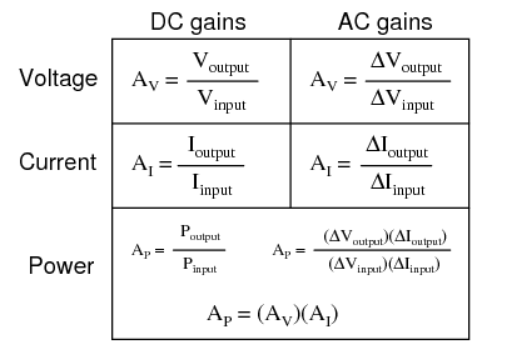
\includegraphics[width=8cm]{Imagenes/gain_amp.png}
    \caption{Distintas Ganancias de un amplificador}
    \label{fig:gain_amp}
\end{figure}

La siguiente ecuación es la mas usada en este capitulo,

\begin{equation}
    A_v=\dfrac{v_o}{V_{in}}
    \label{eqn:av}
\end{equation}





\subsection{Etapas de un amplificador base}
\subsubsection{Amplificador diferencial}
La mayoría de los amplificadores operativos modernos utilizan un extremo frontal de amplificador diferencial. En otras palabras, la primera etapa del amplificador operacional es un amplificador diferencial.

El amplificador diferencial es un circuito que forma parte fundamental de muchos amplificadores y comparadores.

Es un dispositivo que aumenta la diferencia entre dos voltajes de entrada, pero que destruye cualquier voltaje común a dichas entradas. Se trata de un circuito analógico con dos entradas denominadas entrada inversora y entrada no inversora y una sola salida proporcional a la diferencia entre los dos voltajes.

Algunos fabricantes llaman a este instrumento como par diferencial.

En el amplificador diferencial ideal la salida depende de la diferencia de las señales de entrada:

\begin{equation}
    V_o=V_d A_d
\end{equation}

Siendo $V_d$ la señal diferencial y  $A_d$ la ganancia diferencial.

En el amplificador diferencial real la salida depende además de la señal común de ambas entradas:

\begin{equation}
    V_o=V_d A_d+ V_c A_c
\end{equation}

$V_c$ es la señal en modo común
\begin{equation}
    V_c = \dfrac{V_1+V_2}{2}
\end{equation}

$A_c$ es la ganancia en modo común.
A continuación en la figura \ref{fig:diferencial} se muestra la configuración básica de este amplificador.

\begin{figure}[H]
    \centering
    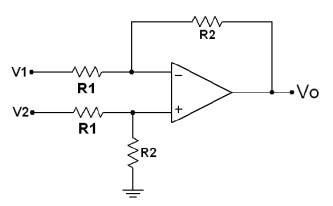
\includegraphics[width=8cm]{Imagenes/diferencial.png}
    \caption{Configuración básica Amplificador Diferencial}
    \label{fig:diferencial}
\end{figure}

Es un montaje simétrico, son dos etapas en emisor común con acoplamiento directo en el emisor.
Las señales de entrada $V_1$ y $V_2$ se aplican en las bases y las señales de salida $V_{o1}$ y $V_{o2}$ se toman en los colectores.
Tenemos:

\begin{align}
    \text{Salida Diferencia:} &  & V_o=V_{o2}-V_{o1} \\
    \text{Salida Asimétrica:} &  & V_o=V_{o2}
\end{align}

\begin{itemize}
    \item \textbf{Ganancia modo diferencial}

          \begin{equation}
              A_d=-\dfrac{V_o}{Z_d}
              \label{eqn:ad}
          \end{equation}


    \item \textbf{Ganancia modo común}

          \begin{equation}
              A_c=-\dfrac{V_o}{Z_c}
              \label{eqn:ac}
          \end{equation}


    \item \textbf{Relación de Rechazo en Modo Común (CMRR)}
          \begin{equation}
              CMRR=\rho=20\cdot log \left| \dfrac{A_d}{A_c}\right|
              \label{eqn:cmrr}
          \end{equation}
\end{itemize}


En la salida diferencial el comportamiento es ideal.
En la salida asimétrica tendremos buen comportamiento si la resistencia $R_E$ es alta ya que con eso conseguimos que $A_c$ sea baja. Cuanto más baja sea $A_c$
más se asemejará al comportamiento ideal.

Para el cálculo de la Relación de rechazo del modo común:

$V_c$ es la señal en modo común

\subsubsection{Amplificador de la etapa elevadora o driver o impulsora}

La etapa de elevación está diseñada para manejar grandes corrientes y voltajes, lo que permite al amplificador operacional manejar cargas pesadas y proporcionar una salida estable y confiable. Esta etapa se compone de transistores bipolares que trabajan en configuración push-pull, lo que significa que un transistor se encarga de manejar la corriente positiva mientras que el otro maneja la corriente negativa. Esto permite una mayor eficiencia y estabilidad en la salida.

La etapa de elevación es fundamental para el funcionamiento del amplificador operacional ya que:

\begin{itemize}
    \item \textbf{Manejo de cargas pesadas}

          La etapa de elevación permite al amplificador operacional manejar cargas pesadas sin perder su capacidad de amplificación.

    \item \textbf{Estabilidad de la salida}

          La etapa de elevación ayuda a mantener la estabilidad de la señal de salida, asegurando que no haya fluctuaciones indeseadas.

    \item \textbf{Amplificación de señales}

          La etapa de elevación es responsable de amplificar la señal de entrada para proporcionar una salida lo suficientemente fuerte para manejar las cargas externas.

\end{itemize}

\subsubsection{Amplificador de potencia}
Un amplificador de potencia es un amplificador electrónico diseñado para aumentar la magnitud de potencia de una señal de entrada.

A diferencia de los amplificadores de voltaje y corriente, un amplificador de potencia está diseñado para impulsar cargas, y se establece como bloque final en un circuito amplificador.

Entre las aplicaciones más frecuentes de un amplificador de potencia destacan:

\begin{itemize}
    \item Medición de valores de impedancia muy bajos.
    \item Medición de impedancia dependiente del voltaje.
    \item Dotar de más potencia en los circuitos durante la medición de impedancia de entrada o de salida.
    \item Generar más energía en entornos ruidosos, como mediciones en convertidores de CC/CC de alta potencia o convertidores de CA/CC.
\end{itemize}

\paragraph{Clases de amplificadores de potencia}

Los amplificadores de potencia más comunes son los que se utilizan en los circuitos de amplificadores de audio y vienen en clases A, B, AB o C.

\subparagraph{Amplificador de potencia clase A:}

En el amplificador de potencia de la clase A, toda la forma de onda de entrada se usa en el proceso de amplificación. Por lo que son los amplificadores de potencia de uso más comunes.

En los amplificadores de potencia de clase A, un único transistor se usa para amplificar las mitades positiva y negativa de la forma de onda. Por otro lado, su ángulo de conducción es de 360º, por lo que los niveles de distorsión de señal son muy inferiores y permiten un mejor rendimiento de alta frecuencia. Sin embargo, una de las principales desventajas de los amplificadores de potencia y especialmente del amplificador de Clase A es que su eficiencia de conversión general es muy baja, ya que las grandes corrientes significan que se pierde una cantidad considerable de energía en forma de calor.

\begin{figure}[H]
    \centering
    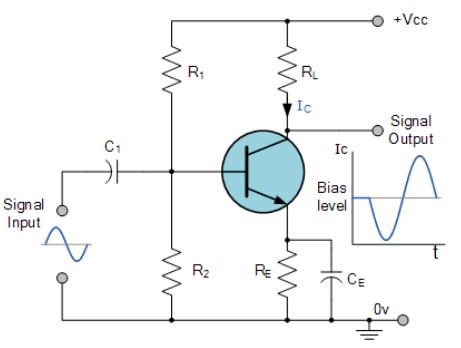
\includegraphics[width=8cm]{Imagenes/potencia_bjt.jpg}
    \caption{Transistor BTJ en configuración Emisor Común para amplificación de CA}
    \label{fig:potencia}
\end{figure}

\subparagraph{Amplificador de potencia clase B o Push and Pull:}

Los amplificadores de Clase B usan dos o más transistores polarizados de tal forma que cada transistor solo conduce durante un medio ciclo (realmente, "casi" medio ciclo) de la onda de entrada. Tienen un rendimiento muy superior a los de Clase A y su diseño no es muy complicado, pero sus aplicaciones se limitan enormemente debido a una característica su propio diseño: una distorsión llamada de "cruce por cero". Aún así, se utilizan incluso en amplificadores que no requieran buena fidelidad y sí facilidad de diseño y rendimiento, como los amplificadores de bocinas y megáfonos de mano.

Para mejorar la eficiencia de potencia total del amplificador de clase A previo, reduciendo la potencia desperdiciada en forma de calor, es posible diseñar el circuito amplificador de potencia con dos transistores en su etapa de salida, produciendo lo que comúnmente se denomina amplificador de clase B; también conocido como configuración de amplificador Push-Pull (empuja-tira en español). Para construir este tipo de amplificador se utilizan necesariamente transistores denominados "complementarios", es decir, de las mismas características eléctricas pero con distintas uniones P-N: si uno es del tipo NPN, el otro ha de ser igual pero de tipo PNP.

\begin{figure}[H]
    \centering
    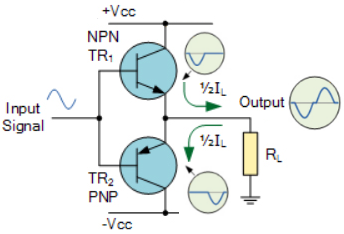
\includegraphics[width=8cm]{Imagenes/clase_b.png}
    \caption{transistores complementarios BJT en funcionamiento clase B, configuración Push-Pull}
    \label{fig:clase_b}
\end{figure}


Los amplificadores Push-Pull utilizan transistores complementarios de potencia, que reciben la misma señal de entrada que es igual en magnitud, pero en fase opuesta entre sí. Esto da lugar a que un transistor solamente amplifica la mitad o 180º del ciclo de la onda de entrada; mientras que el otro transistor amplifica la otra mitad o restante 180º del ciclo de onda de entrada.

Conjuntamente, estas “dos mitades” amplificadas cada una por un transistor, "excitan" o "atacan" la carga o resistencia de salida, dando lugar en ella a la señal completa amplificada.

Por consiguiente, el ángulo de conducción para este tipo de circuito amplificador es escasamente inferior a 180º o $50\%$ de la señal de entrada (para cada transistor). Este efecto de empujar y tirar de los semi ciclos alternos por los transistores da a este tipo de circuito su divertido nombre "push-pull", pero en general se lo conoce como el amplificador de clase B.

Realmente los transistores en un amplificador de clase B no llegan al conducir el $50\%$, ya que ambos necesitan tener una polarización al menos de 0.65 V Emisor-Base para empezar a conducir y amplificar. Esto supone que de la señal de entrada, en los primeros 0.65 V. (positivos y negativos), la señal de salida va a estar a "0". Y sólo cuando en la entrada se superen los 0.65 V. E-B podrá empezar a amplificar la salida. Esto, al final, produce inevitablemente una falta de amplificación en torno a los valores cercanos a "0" V. denominada "distorsión de paso por cero" o "distorsión de cruce", característica de los amplificadores en Clase B.

\begin{figure}[H]
    \centering
    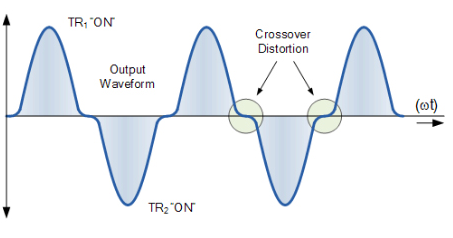
\includegraphics[width=10cm]{Imagenes/crossover.png}
    \caption{formas de señal de saldia debida a la "distorsión de cruce"    o     "de paso por 0" en un amplificador Clase B, Push-Pull}
    \label{fig:crossover}
\end{figure}

\subparagraph{Amplificador de potencia clase AB:}

Un amplificador de clase AB está polarizado de modo que la corriente de salida fluye durante menos de un ciclo completo de la forma de onda de entrada pero más de medio ciclo. La implementación de los amplificadores de Clase AB es muy similar a las configuraciones de Clase B estándar en que utiliza dos transistores de conmutación como parte de una etapa de salida complementaria con cada transistor conduciendo en semi-ciclos opuestos de la forma de onda de entrada antes de combinarse en la carga.

Por lo tanto, al permitir que ambos transistores de conmutación conduzcan corriente al mismo tiempo durante un período muy corto, la forma de onda de salida durante el período de cruce cero se puede suavizar sustancialmente reduciendo la distorsión de cruce asociada con el diseño del amplificador de clase B. Entonces el ángulo de conducción es mayor de 180° pero mucho menor de 360°.

\begin{figure}[H]
    \centering
    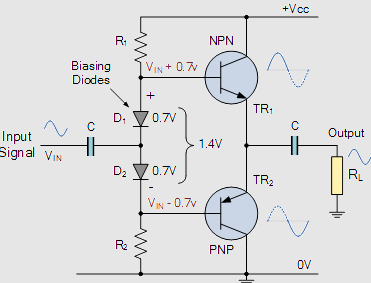
\includegraphics[width=10cm]{Imagenes/clase_ab.png}
    \caption{Esquemático de un amplificador clase AB, polarizado por diodos }
    \label{fig:clase_ab}
\end{figure}

Una configuración de amplificador de clase AB es más eficiente que un amplificador de clase A pero un poco menos eficiente que la de un clase B debido a la pequeña corriente de reposo necesaria para polarizar los transistores justo por encima del límite. Sin embargo, el uso de polarización incorrecta puede causar picos de distorsión cruzada que producen una peor condición.

Dicho esto, los amplificadores de clase AB son uno de los diseños de amplificadores de potencia de audio más preferidos debido a su combinación de una eficiencia razonablemente buena y una salida de alta calidad, ya que tienen una baja distorsión de cruce y una alta linealidad similar al diseño de amplificador de clase A.

\subparagraph{Amplificador de potencia clase C:}

Los amplificadores de potencia en clase C parten de la premisa siguiente: no se trata de amplificar con calidad la señal de entrada, se trata simplemente de amplificar la señal de entrada de modo que a la salida se obtenga el máximo rendimiento posible pero sólo para un rango de frecuencias muy reducido, en torno a una de "resonancia".

Son amplificadores que desde luego no sirven para señales de audio, por la distorsión. Su campo de aplicación está en las telecomunicaciones, en radiofrecuencia, F, donde se requiere un incremento en el nivel de potencia y no se requiere linealidad entre la tensión de entrada y tensión de salida. Los amplificadores Clase C pueden ser modulados en amplitud para amplificar una portadora modulada en frecuencia.

\begin{figure}[H]
    \centering
    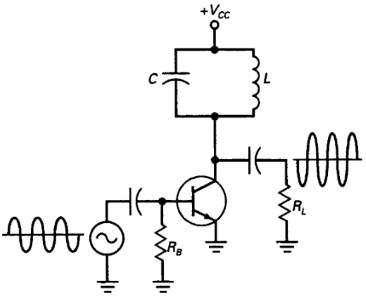
\includegraphics[width=7cm]{Imagenes/amplificador resonante01.png}
    \caption{etapa amplificadora a transistor BJT con circuito tanque resonante }
    \label{fig:clase_c}
\end{figure}

Este tipo de amplificadores se reconoce porque tienen, en lugar de la resistencia de colector típica, un "circuito tanque" formado por un condensador y bobina diseñados para que en un estrecho margen de frecuencias entren en sintonía -por lo que también se le llama "circuito resonante"-y, modificando la impedancia del circuito L-C produzcan la conducción del transistor. Es por eso que a este tipo de circuitos les llama amplificadores "resonantes" o "sintonizados".

En torno a la frecuencia de resonancia, estos amplificadores obtienen una ganancia alta; fuera de esta frecuencia, la amplificación es muy reducida y el consumo es mínimo.


\begin{figure}[H]
    \centering
    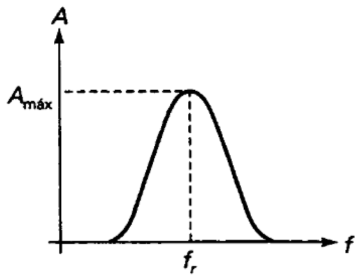
\includegraphics[width=7cm]{Imagenes/amplificador resonante02.png}
    \caption{etapa amplificadora a transistor BJT con circuito tanque resonante }
    \label{fig:campana de gauss}
\end{figure}

\subsubsection{Amplificadores de varias etapas}

La conexión más utilizada para amplificadores de varias etapas:

\paragraph{\textbf{Conexión en cascada}}

\begin{figure}[H]
    \centering
    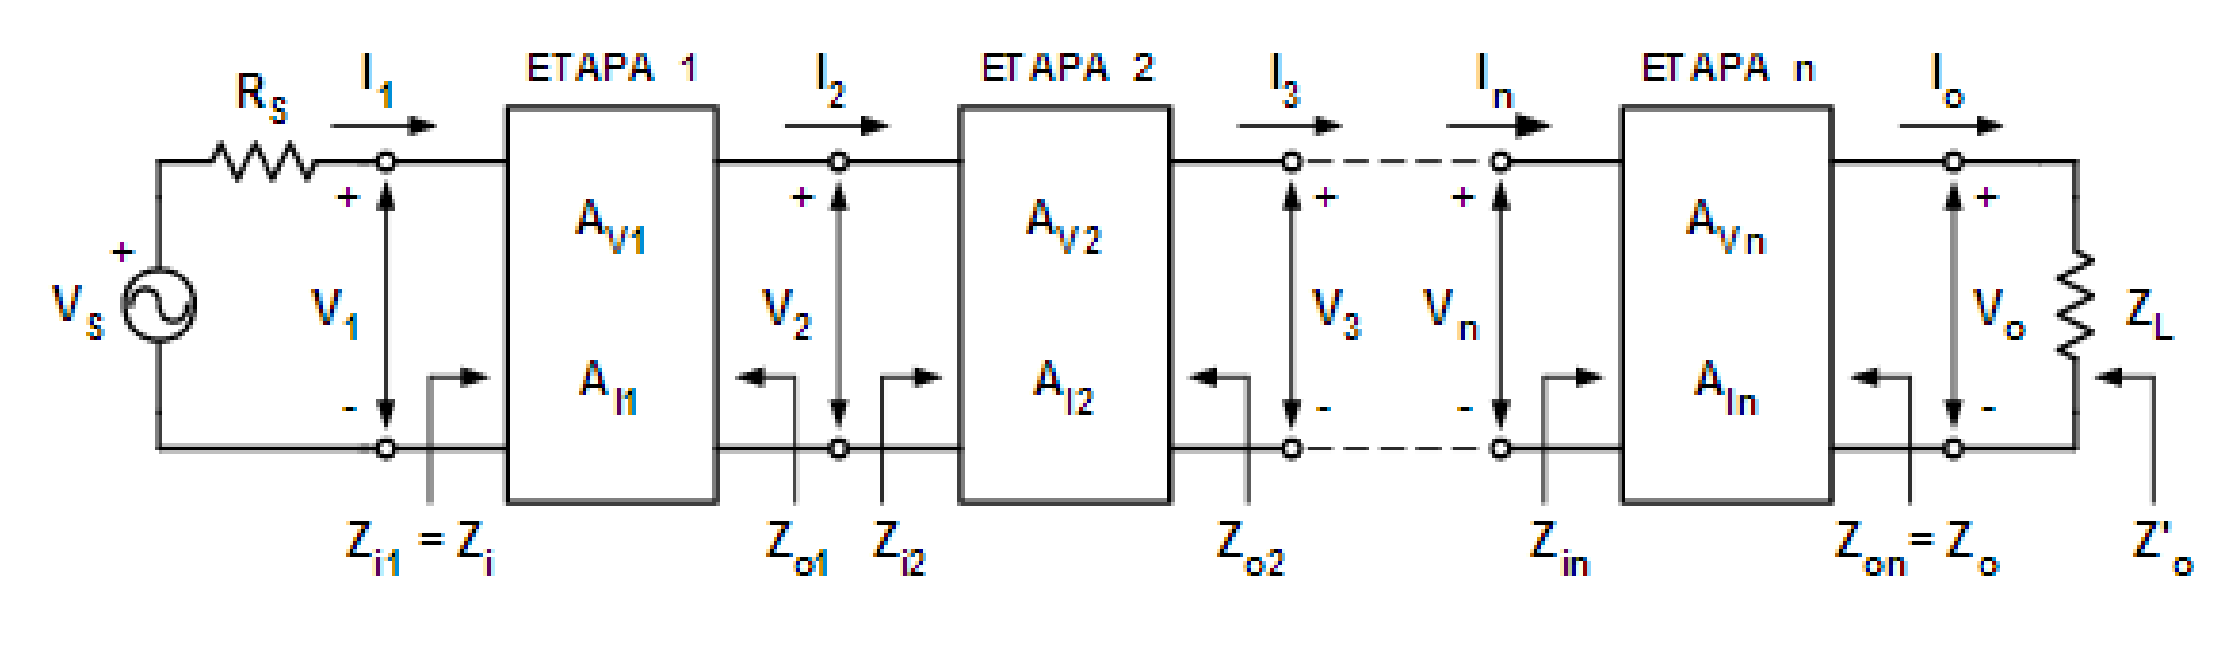
\includegraphics[width=15cm]{Imagenes/amp_base.png}
    \caption{Conexión en cascada de varios amplificadores}
    \label{fig:cascada}
\end{figure}

Hay influencias de una etapa sobre otra, la señal de salida de cada etapa se aplica como señal de entrada de la siguiente.

Las ganancias de tensión de cada etapa y sus impedancias teniendo en cuenta lo siguiente, serán:
\begin{gather}
    A_v= A_{v1}A_{v2}...A_{vn}
    \label{eqn:avt}
\end{gather}

\begin{align*}
     & \text{Impedancia de entrada} &  & Z_in= Z_n        \\
     & \text{Impedancia de salida}  &  & Z_o= Z_{On}      \\
     &                              &  & Z'_o= Z_{L}||Z_o
\end{align*}

Nosotros nos centraremos en los amplificadores de alterna, hay varios tipos de acoplamientos entre etapas, aquí nos centraremos en el acoplamiento RC.

El acoplamiento entre etapas es mediante un condensador. Como se indico anteriormente sobre los condensadores de acople y desacople.

\newpage

\subsection{Respuesta en frecuencia}

A respuesta en frecuencia de un amplificador operacional en lazo cerrado o lazo abierto se define como el límite de alta frecuencia y el límite de baja frecuencia. En estos límites, la ganancia de voltaje se reduce un 0.707 del valor máximo de voltaje, en el rango de frecuencia útil.
El ancho de banda para pequeña señal es la diferencia entre el límite de alta frecuencia y el límite de baja frecuencia. Además se debe agregar que:

\begin{itemize}
    \item \textbf{Para frecuencias medias}, los condensadores de acople y desacople se comportan como un cable, es decir, un cortocircuito.
    \item \textbf{Para frecuencias altas}, las limitaciones en frecuencia de los dispositivos activos condicionan 1a frecuencia máxima de operación del amplificador.
    \item \textbf{Para frecuencias bajas}, el efecto de los condensadores de acoplo y desacoplo es importante.
\end{itemize}

\subsubsection{Análisis de respuesta en frecuencia}

\begin{itemize}
    \item \textbf{Frecuencias bajas:} Se toma en cuenta el condensador que se va a estudiar en bajas frecuencias, siendo estos los de acople, desacople y bypass. Al escoger el condensador, ese se reemplaza por una fuente de prueba y los demás capacitores se cortocircuitan y los de alta frecuencia son un abierto. Así, se puede hallar la impedancia equivalente. Se hace uso de la ecuación \ref{eqn:wl}.

          \begin{equation}
              w_{p_n}=\dfrac{1}{C_nZ_{eq}}
              \label{eqn:wl}
          \end{equation}

    \item \textbf{Frecuencias altas:} Se toma en cuenta los capacitores que estén conectados entre base y emisor o base y colector, con un valor de capacitancia bastante bajo, cercano a los $\si{pF}$. Se aplica el teorema de miller, que es la ecuación \ref{eqn:C_eq} y su frecuencia de corte superior siendo la ecuación \ref{eqn:wh}.

          \begin{equation}
              w_{H}=\dfrac{1}{C_{eq}Z_{in}}
              \label{eqn:wh}
          \end{equation}

    \item \textbf{Frecuencia de corte superior total}
          \begin{equation}
              w_t=\beta \cdot f_H
              \label{eqn:wt}
          \end{equation}
\end{itemize}



\subsection{Realimentación en un amplificador}

La realimentación consiste e11 combinar una muestra de la señal de salida del amplificador con la señal de entrada, de modo tal que se modifican las características generales del sistema. Puede ser positiva o negativa.

\subsubsection{Realimentación negativa}

La realimentación es negativa cuando el valor de la señal de salida es menor que sin la realimentación. Para ello, la serial de salida que se toma como muestra es aplicada opuesta en fase a la serial de entrada.

La realimentación negativa disminuye la ganancia del amplificador y a pesar de ello, la inmensa mayoría de los amplificadores utilizan esta variante de realimentación debido a las muchas ventajas que se obtienen con la aplicación de este principio, tales como el aumento
de la estabilidad y el ancho de banda, 1a disminución de las distorsiones de frecuencia y de no linealidad así como del ruido y el cambio en las resistencias de entrada y salida. Todo esto incrementa notablemente la calidad y versatilidad de los amplificadores.

Los cambios provocados por el envejecimiento de los componentes y dispositivos, su reemplazo u otras causas, las variaciones de temperatura, etcétera, se reflejan en las alteraciones que puede sufrir la ganancia de un amplificador con relación a su valor original. Tales
alteraciones son de hecho reducidas con la realimentación negativa, a tal extremo que su ganancia puede llegar a depender solamente de las características de la red de realimentación, cuando la ganancia de lazo es mucho mayor que la unidad.


\subsubsection{frecuencia de corte inferior en realimentación no inversora}
\begin{equation}
    w_{L_{fb}}=\dfrac{w_L}{A_{fb}}=\dfrac{w_L}{1+\dfrac{R_f}{R_s}}
    \label{eqn:wlfb}
\end{equation}
\subsubsection{frecuencia de corte superior en realimentación no inversora}
\begin{equation}
    w_{H_{fb}}=w_H(A_{fb})=w_L(1+\dfrac{R_f}{R_s})
    \label{eqn:whfb}
\end{equation}

\subsubsection{Ganancia en retroalimentación de un no inversor}
\begin{equation}
    A_{fb}=1+\dfrac{R_f}{R_s}
    \label{eqn:afb}
\end{equation}


\subsubsection{Impedancias de entrada en realimentación negativa o degenerativa}
\begin{equation}
    Z_{in}=Z_d\left(1 +\dfrac{A_{fm}}{A_{fb}}\right)
    \label{eqn:zinfb}
\end{equation}
\subsubsection{Impedancias de salida en realimentación negativa o degenerativa}
\begin{equation}
    Z_{o}=\left(\dfrac{Z_o}{\dfrac{A_{fm}}{A_{fb}}}\right)
    \label{eqn:zofb}
\end{equation}
\subsubsection{Realimentación positiva}

La realimentación es positiva cuando el valor de la señal de salida es mayor que sin la realimentación. Esto se logra cuando la señal de salida que se toma como muestra es
aplicada en fase con la señal de entrada.

El resultado de la realimentación positiva es contrario a la realimentación negativa, es decir se incrementa el ruido, la ganancia y la distorsión, disminuyendo el ancho de banda y la estabilidad, por lo cual este efecto no es aconsejable para los amplificadores, sin embargo, puede ser aprovechado con gran eficacia en los circuitos osciladores.

\subsection{Método de amplificador desvanecido}

El método consiste en añadir una ganancia adicional variable a la señal recibida, dependiendo de la calidad de la señal, para compensar la atenuación y mejorar la relación señal—ruido. Esta ganancia adicional se calcula en función de la retroalimentación recibida de la señal de error, que se obtiene comparando la señal recibida con la señal transmitida originalmente.

El Amplificador Desvanecido puede ser implementado de varias maneras, incluyendo la retroalimentación de la señal de en un circuito de control de ganancia, o utilizando
técnicas de procesamiento digital de señales para ajustar la ganancia en tiempo real.

Este método es particularmente útil en sistemas de comunicación inalámbrica de alta frecuencia, como los sistemas de comunicación móvil, donde la atenuación de la señal debido a la propagación en el medio ambiente puede ser significativa y afectar la calidad de la señal
recibida.

\subsection{Método de Blackman}

Es una técnica utilizada para calcular la impedancia de entrada de un amplificador.Esta técnica se basa en la medición de la tensión de entrada y corriente de entrada del
amplificador, y en el uso de una red de resistencias y capacitores para modelar la impedancia
de entrada del amplificador.

El método de Blackman utiliza una red de dos resistencias y un capacitor, conectados en serie con la entrada del amplificador. La tensión de entrada se mide a través de una de las resistencias, mientras que la corriente de entrada se mide a través de la otra resistencia.

A partir de estas mediciones, se puede calcular la impedancia de entrada del amplificador utilizando la ley de Ohm y la ley de Kirchhoff.

La ventaja del método de Blackman es que permite obtener una medida precisa de la impedancia de entrada del amplificador en una amplia gama de frecuencias. Además, esta
técnica es relativamente sencilla y económica de implementar, lo que la hace adecuada para su uso en aplicaciones practicas.

Sin embargo, es importante tener en cuenta que el método de Blackman asume que la impedancia de entrada del amplificador es constante en toda la gama de frecuencias de
interés, lo cual puede no ser cierto en algunos casos.

\subsection{Formula de propagación de incertidumbres}

Para calcular la incertidumbre en un resultado calculado indirectamente, como \( V_{CE} = V_C - V_E \), puedes utilizar la fórmula de propagación de incertidumbres. Esta fórmula se aplica cuando tienes dos o más cantidades medidas y deseas determinar la incertidumbre en una cantidad derivada a partir de ellas. La fórmula general es:

\[ \Delta Q = \sqrt{\left(\frac{\partial Q}{\partial A} \Delta A\right)^2 + \left(\frac{\partial Q}{\partial B} \Delta B\right)^2 + \ldots} \]

Donde:
- \( Q \) es la cantidad derivada (en este caso, \( V_{CE} \)),
- \( A, B, \ldots \) son las cantidades medidas (en este caso, \( V_C \) y \( V_E \)),
- \( \Delta A, \Delta B, \ldots \) son las incertidumbres asociadas a las cantidades medidas, y
- \( \frac{\partial Q}{\partial A}, \frac{\partial Q}{\partial B}, \ldots \) son las derivadas parciales de \( Q \) con respecto a \( A, B, \ldots \).

En este caso, como \( V_{CE} = V_C - V_E \), las derivadas parciales son simples:

\[ \frac{\partial V_{CE}}{\partial V_C} = 1, \quad \frac{\partial V_{CE}}{\partial V_E} = -1 \]

Entonces, la fórmula para la incertidumbre en \( V_{CE} \) sería:

\[ \Delta V_{CE} = \sqrt{\left(\Delta V_C\right)^2 + \left(\Delta V_E\right)^2} \]

Sustituyendo los valores dados:

\[ \Delta V_{CE} = \sqrt{(0.1)^2 + (0.02)^2} \]

\[ \Delta V_{CE} = \sqrt{0.01 + 0.0004} \]

\[ \Delta V_{CE} \approx \sqrt{0.0104} \]

\[ \Delta V_{CE} \approx 0.102 \volt \]

Entonces, la incertidumbre en \( V_{CE} \) es aproximadamente \( \pm 0.102 \volt \). Puedes informar el resultado como \( V_{CE} = 1.06 \pm 0.102 \volt \).

\subsection{Error Porcentual}

Porcentaje de error (\% de error), también conocido como porcentaje de error, es una medida de cuánto un valor difiere del valor esperado. Puede usarse para determinar qué tan lejos está un valor esperado de otro valor, pero a menudo se usa en el contexto de experimentos científicos.

Se puede expresar en la siguiente ecuación:

\begin{equation}
    E_r =\dfrac{|Valor_{experimental}-Valor_{teorico}|}{Valor_{teorico}} \cdot  100
    \label{eqn:error}
\end{equation}

\subsection{Impedancia de entrada/diferencial (medición indirecta)}

La siguiente ecuación se lleva a cabo debido a un divisor de tensión realizado de la siguiente manera:

\begin{figure}[H]
    \centering
    \begin{circuitikz}[transform shape,scale=1]

  \draw (2.25,-2.25) to[short,-*] (2.25,-2.25) coordinate (X0);
  \def\OpAmpsopamp(#1)#2#3{%
    \begin{scope}[#1,transform canvas={scale=1}]
      \draw (0.0,0.25) -- (1.0,-0.25);
      \draw (0.0,-0.75) -- (1.0,-0.25);
      \draw (0.0,0.25) -- (0.0,-0.75);
      \draw (0.0625,0.0) -- (0.1875,0.0);
      \draw (0.0625,-0.5) -- (0.1875,-0.5);
      \draw (0.125,-0.5625) -- (0.125,-0.4375);
      \draw (0.5,0.25) coordinate (#2 text);
      \draw (0.0,0.0) coordinate (#2 X0);
      \draw (0.0,-0.5) coordinate (#2 X1);
      \draw (1.0,-0.25) coordinate (#2 X2);
    \end{scope}
    \draw (#2 text) node[right] {#3};
  }
  \draw (2.25,-3.5) node[ground] {} ;
  \node[right] at (-2.0,-2.25) {Vg} ;
  \node[right] at (2,-2.0) {Vi} ;
  \node[right] at (5.5,-2.5) {Vo} ;
  \OpAmpsopamp (shift={(3.5,-2.25)},rotate=0  ) {B0} {Amp. Op};
  \draw (X0) to[R,l=Rp] (-0.5,-2.25) ;
  \draw (B0 X0) to[short,-] (X0) ;
  \draw (5.5,-2.5) to[short,-] (5.0,-2.5) ;
  \draw (B0 X1) to[short,-] (2.25,-2.75) ;
  \draw (2.25,-3.5) to[short,-] (2.25,-2.75) ;
  \draw (-0.5,-2.25) to[short,-] (-1.0,-2.25) ;
  \draw (5.0,-2.5) to[short,-] (B0 X2) ;

\end{circuitikz}
    \caption{Circuito simplificado de un amplificador para hallar su impedancia de entrada}
    \label{fig:zin_amp}
\end{figure}

\begin{gather}
    V_i=V_g \, \dfrac{Z_{d}}{Z_{d}+R_p} \nonumber \\[0.2cm]
    V_iZ_{d}+V_iR_p = V_gZ_{d} \nonumber \\[0.2cm]
    V_gZ_{d} - V_iZ_{d} = V_iR_p  \nonumber \\[0.2cm]
    Z_{d} = V_i \dfrac{R_p}{V_g-V_i}  \label{eqn:zin}
\end{gather}

\subsection{Impedancia de entrada/modo Común (medición indirecta)}

Se visualiza el modelo del amplificador para sus impedancias de entrada en modo común, donde se usará la siguiente ecuación:

\begin{gather}
    V_i=V_g \,\dfrac{Z_{c}}{2} \dfrac{1}{\dfrac{Z_{c}}{2}+R_p} \nonumber \\[0.2cm]
    V_i=V_g \, \dfrac{Z_{c}}{2} \dfrac{1}{\dfrac{Z_{c}+2R_p}{2}} \nonumber \\[0.2cm]
    V_iZ_{c}+2V_iR_p = V_gZ_{c} \nonumber \\[0.2cm]
    V_gZ_{c} - V_iZ_{c} = 2V_iR_p  \nonumber \\[0.2cm]
    Z_{c} = 2V_i \dfrac{R_p}{V_g-V_i}  \label{eqn:zc}
\end{gather}

\subsection{Impedancia de salida (medición indirecta)}

La siguiente ecuación, al igual que la impedancia de entrada se lleva a cabo con un divisor de tensión, como se verá a continuación:

\begin{figure}[H]
    \centering 
\ctikzset{tripoles/mos style/arrows} 
\begin{circuitikz}[transform shape,scale=1] 
 
\def\OpAmpsopamp(#1)#2#3{%
  \begin{scope}[#1,transform canvas={scale=1}]
  \draw (0.0,0.25) -- (1.0,-0.25);
  \draw (0.0,-0.75) -- (1.0,-0.25);
  \draw (0.0,0.25) -- (0.0,-0.75);
  \draw (0.0625,0.0) -- (0.1875,0.0);
  \draw (0.0625,-0.5) -- (0.1875,-0.5);
  \draw (0.125,-0.5625) -- (0.125,-0.4375);
  \draw (0.5,0.25) coordinate (#2 text);
  \draw (0.0,0.0) coordinate (#2 X0);
  \draw (0.0,-0.5) coordinate (#2 X1);
  \draw (1.0,-0.25) coordinate (#2 X2);
  \end{scope}
  \draw (#2 text) node[right] {#3};
}
\draw (2.25,-3.5) node[ground] {} ;
\node[right] at (5.5,-2.5) {Vosc} ;
\node[right] at (1.50,-2.25) {Vi} ;
\OpAmpsopamp (shift={(3.5,-2.25)},rotate=0  ) {B0} {AmpOp};
\draw (B0 X0) to[short,-] (2.875,-2.25) ;
\draw (5.5,-2.5) to[short,-] (5.0,-2.5) ;
\draw (B0 X1) to[short,-] (2.25,-2.75) ;
\draw (2.25,-3.5) to[short,-] (2.25,-2.75) ;
\draw (2.875,-2.25) to[short,-] (2.25,-2.25) ;
\draw (5.0,-2.5) to[short,-] (B0 X2) ;

\end{circuitikz}
    \caption{Circuito simplificado de un amplificador para medir su voltaje sin carga, medida para hallar su impedancia de salida}
    \label{fig:zout_amp1}
\end{figure}

\begin{figure}[H]
    \centering
    \ctikzset{tripoles/mos style/arrows} 
\begin{circuitikz}[transform shape,scale=1] 
 
\draw (5.0,-2.5) to[short,-*] (5.0,-2.5) coordinate (X0);
\def\OpAmpsopamp(#1)#2#3{%
  \begin{scope}[#1,transform canvas={scale=1}]
  \draw (0.0,0.25) -- (1.0,-0.25);
  \draw (0.0,-0.75) -- (1.0,-0.25);
  \draw (0.0,0.25) -- (0.0,-0.75);
  \draw (0.0625,0.0) -- (0.1875,0.0);
  \draw (0.0625,-0.5) -- (0.1875,-0.5);
  \draw (0.125,-0.5625) -- (0.125,-0.4375);
  \draw (0.5,0.25) coordinate (#2 text);
  \draw (0.0,0.0) coordinate (#2 X0);
  \draw (0.0,-0.5) coordinate (#2 X1);
  \draw (1.0,-0.25) coordinate (#2 X2);
  \end{scope}
  \draw (#2 text) node[right] {#3};
}
\draw (2.25,-3.5) node[ground] {} ;
\node[right] at (5.5,-2.5) {Vocc} ;
\node[right] at (1.50,-2.25) {Vi} ;
\draw (5.0,-3.75) node[ground] {} ;
\OpAmpsopamp (shift={(3.5,-2.25)},rotate=0  ) {B0} {AmpOp};
\draw (X0) to[R,l=Rp] (5.0,-3.75) ;
\draw (B0 X0) to[short,-] (2.875,-2.25) ;
\draw (X0) to[short,-] (B0 X2) ;
\draw (5.5,-2.5) to[short,-] (X0) ;
\draw (B0 X1) to[short,-] (2.25,-2.75) ;
\draw (2.25,-3.5) to[short,-] (2.25,-2.75) ;
\draw (2.875,-2.25) to[short,-] (2.25,-2.25) ;

\end{circuitikz}
    \caption{Circuito simplificado de un amplificador para medir su voltaje con carga, medida para hallar su impedancia de salida}
    \label{fig:zout_amp2}
\end{figure}

Como se observa en la figura \ref{fig:zout_amp1} y \ref{fig:zout_amp2}, luego de realizar esas medidas se realiza un divisor de tensión que permite la medición de su impedancia.

\begin{gather}
    V_{occ}=\dfrac{V_{oscR_p}}{R_p + Z_o} \nonumber \\[0.2cm]
    Z_oV_{occ} + V_{occ}R_p=V_{osc}R_p \nonumber \\[0.2cm]
    Z_o= \dfrac{V_{osc}R_p - V_{occ}R_p}{V_{occ}} \label{eqn:zo}
\end{gather}


\subsection{Uso de PPM en la Incertidumbre de la Medición del Intervalo de Tiempo en un Osciloscopio}

En el ámbito de la electrónica y la instrumentación, la precisión y la exactitud de las mediciones son cruciales. Los osciloscopios, herramientas esenciales en la medición de señales eléctricas, requieren una comprensión detallada de sus especificaciones para asegurar resultados confiables. Una de las métricas importantes en estos dispositivos es la incertidumbre de la medición del intervalo de tiempo, donde el concepto de partes por millón (ppm) juega un papel significativo.

\subsubsection{Concepto de PPM (Partes por Millón)}

PPM es una unidad de medida que expresa una proporción como una fracción de un millón. Es comúnmente utilizada en campos donde se requieren mediciones extremadamente precisas, como en la electrónica, para representar pequeñas variaciones o errores relativos en una cantidad medida. En el contexto de un osciloscopio, ppm se emplea para cuantificar la exactitud del intervalo de tiempo medido, relacionando el error relativo con la lectura.

Matemáticamente, 1 ppm se define como:

\[
    1 \, \text{ppm} = \frac{1}{1,000,000} = 10^{-6}
\]

\subsubsection{Incertidumbre de la Medición del Intervalo de Tiempo}

La incertidumbre en la medición del intervalo de tiempo de un osciloscopio es la desviación esperada de la medida real debido a las limitaciones del dispositivo. Esta incertidumbre se compone de varios factores, incluyendo el intervalo de muestreo, la resolución del dispositivo, y un componente proporcional a la lectura expresado en ppm.

En el manual de un osciloscopio típico, la incertidumbre de la medición del intervalo de tiempo (\(\Delta T\)) se especifica como:

\[
    \Delta T = \pm \left( \text{intervalo de muestreo} + 50 \text{ ppm} \times \text{lectura} + 0.6 \text{ ns} \right)
\]

\subsubsection{Desglose de la Fórmula}

\begin{enumerate}
    \item \textbf{Intervalo de Muestreo}

          Es el tiempo entre dos muestras consecutivas que toma el osciloscopio. A menor intervalo de muestreo, mayor es la precisión temporal del dispositivo.

    \item \textbf{50 ppm \(\times\) Lectura}

          Este término indica que el error relativo es proporcional a la lectura del intervalo de tiempo. La constante de 50 ppm refleja la precisión del osciloscopio en términos de ppm. Para convertir 50 ppm a una fracción decimal:

          \[
              50 \, \text{ppm} = 50 \times 10^{-6} = 0.00005
          \]

          Por lo tanto, si la lectura es de 100 ns, el error debido a este término sería:

          \[
              0.00005 \times 100 \, \text{ns} = 0.005 \, \text{ns}
          \]

    \item 0.6 ns

          Un componente fijo de la incertidumbre que representa errores sistemáticos adicionales en la medición.

\end{enumerate}

\subsubsection{Importancia en Aplicaciones Electrónicas}

Comprender la incertidumbre de la medición es esencial para ingenieros y técnicos que dependen de los osciloscopios para diseñar, probar y verificar circuitos electrónicos. La especificación en ppm permite evaluar y comparar la precisión de diferentes osciloscopios, asegurando que las mediciones sean suficientemente precisas para las aplicaciones específicas.

\newpage

    
    \section{Dispositivos} \label{sec:dispositivos}

    La transmisión de energía eléctrica a través de líneas de transmisión implica inevitablemente la disipación de una parte de esa energía en forma de calor, radiación y otras pérdidas. Estas pérdidas energéticas, que pueden reducir la eficiencia del sistema y generar problemas operativos, son causadas por diversos factores relacionados con las características de la línea, los materiales utilizados y las condiciones ambientales. Para cuantificar y analizar estas pérdidas de manera precisa, es fundamental emplear dispositivos de medición especializados. En esta sección, exploraremos en detalle los distintos instrumentos utilizados para medir las pérdidas en líneas de transmisión en los diferentes tipos de perdidas antes mencionados, lo que permitirá una evaluación exhaustiva del desempeño de los sistemas de transmisión y la identificación de áreas de mejora.

    \subsection{Medición de pérdidas en el conductor (Efecto Joule)}

        Las pérdidas en los conductores de una línea de transmisión, que son principalmente pérdidas resistivas (efecto Joule), pueden medirse utilizando diversos métodos, tanto directos como indirectos, dependiendo del equipo disponible, el tipo de línea, y la precisión deseada. A continuación te explico algunas de las formas más comunes para medir estas pérdidas:

        \subsubsection{Medición de la caída de voltaje}

            Uno de los métodos más sencillos para medir las pérdidas resistivas en un conductor es medir la caída de voltaje entre dos puntos de la línea de transmisión, generalmente entre la fuente y la carga.

            La pérdida resistiva puede calcularse como:

            \begin{gather}
                P_{perdida} = I \cdot \Delta V \label{eq:potencia_perd}
            \end{gather}

            Donde:
            \begin{align*}
                I &= \text{es la corriente que fluye por el conductor.} \\[0.2cm]
                \Delta V &= \text{es la caída de voltaje entre los dos puntos del conductor (medida con un voltímetro).}
            \end{align*}

            \begin{itemize}
                \item \textbf{Ventajas} 

                    Método directo y sencillo.  

                
                \item \textbf{Desventajas}

                    Es más útil para distancias cortas y situaciones donde el voltaje no es muy elevado.
            \end{itemize}

        \subsubsection{Medición de la resistencia del conductor y cálculo de pérdidas}

            Otra forma común de cuantificar las pérdidas resistivas en un conductor es medir la resistencia del conductor y luego calcular las pérdidas a partir de la corriente que fluye por el conductor.

            Las pérdidas resistivas se calculan como:

            \begin{gather}
                P_{resistivas} = I^2 R \label{eq:pot_resistiva}
            \end{gather}

            Donde:

            \begin{align*}
                I&= \text{es la corriente que circula por el conductor.}
                R & = \text{ es la resistencia del conductor.}
            \end{align*}

            \paragraph{Proceso:}
                \begin{enumerate}
                    \item Mide la resistencia del conductor mediante un ohmímetro o calculando su resistencia a partir de las propiedades conocidad del material.

                    \begin{gather}
                        R = \rho \dfrac{L}{A} \label{eq:rho}
                    \end{gather}

                    \item Mide la corriente que circula por el conductor.

                    \item Aplicar la fórmula \ref{eq:pot_resistiva} para calcular las pérdidas.
                \end{enumerate}

            \begin{itemize}
                \item \textbf{Ventaja}

                    Método preciso para pérdidas resistivas.

                \item \textbf{Desventaja}

                    Requiere conocer o medir la resistencia exacta del conductor, lo que puede ser complicado si las condiciones de temperatura varían, ya que la resistividad de los materiales cambia con la temperatura.
            \end{itemize}

        \subsubsection{Medición directa de la potencia de entra y salida}

            Este método consiste en medir la potencia de entrada en un extremo de la línea de transmisión y la potencia de salida en el otro extremo. La diferencia entre ambas potencias representa las pérdidas totales en la línea, incluidas las pérdidas resistivas en el conductor.

            \begin{gather}
                P_{perdida} = P_{entrada} - P_{salida} \label{eq:pot_perdida_2}
            \end{gather}

            \begin{itemize}
                \item \textbf{Ventajas}

                    Este método permite obtener una visión global de las pérdidas en la línea.

                    
                \item \textbf{Desventajas}

                    Las mediciones incluyen todas las pérdidas, por lo que no es fácil separar las pérdidas resistivas de otras.
                    
            \end{itemize}

        \subsubsection{Medición de la temperatura del conductor}

             Las pérdidas resistivas en los conductores provocan un aumento de la temperatura debido al efecto Joule. Midiendo el incremento de temperatura en el conductor, se puede estimar la potencia disipada.

             \paragraph{Proceso}

                \begin{enumerate}
                    \item Utiliza un termómetro infrarrojo o sensores de temperatura para medir la temperatura del conductor en condiciones de operación.
                    
                    \item Compara la temperatura medida con la temperatura ambiente o la temperatura del conductor cuando no circula corriente.
                    
                    \item Utiliza las propiedades térmicas del conductor para calcular la energía disipada como calor, lo que te da una idea de las pérdidas resistivas.
                    
                \end{enumerate}


            \begin{itemize}
                \item \textbf{Ventaja}
                
                     Es una forma indirecta de medir las pérdidas que no requiere desconectar la línea.

                     
                \item \textbf{Desventaja}

                     Depende de una buena calibración y comprensión del entorno de operación (pérdidas adicionales debidas a la radiación térmica, convección, etc.).
            \end{itemize}

        \subsubsection{Medición mediante técnicas de reflectometría (TDR)}

            La reflectometría en el dominio del tiempo (TDR) es una técnica utilizada para detectar fallos o cambios en la impedancia de una línea de transmisión, lo cual puede ayudar a identificar zonas con alta resistencia o pérdidas significativas.

            \paragraph{Proceso}

                \begin{enumerate}
                    \item Se envía un pulso de corriente o voltaje a lo largo del conductor.
                    
                    \item Se mide el tiempo que tarda el pulso en reflejarse desde los extremos o puntos de discontinuidad en la línea.
                    
                    \item Las reflexiones indican cambios en la impedancia que pueden estar asociados a pérdidas resistivas o defectos en la línea.
                \end{enumerate}

            \begin{itemize}
                \item \textbf{Ventaja}

                    Detecta pérdidas no uniformes a lo largo del conductor, como puntos calientes o conexiones defectuosas.
                    
                \item \textbf{Desventaja}

                    Requiere equipo especializado y es más útil para diagnósticos y mantenimiento que para una medición continua de pérdidas resistivas.
            \end{itemize}

        \subsubsection{Medición de pérdidas mediante análisis armónico}

            Las pérdidas resistivas pueden aumentar en presencia de armónicos, especialmente en sistemas de transmisión de corriente alterna (CA). Midiendo los armónicos presentes en la línea, se puede estimar cómo los armónicos contribuyen a las pérdidas adicionales en los conductores.

            \paragraph{Proceso}

                \begin{enumerate}
                    \item Se usa un analizador de armónicos para medir la distorsión de la forma de onda de la corriente en el conductor.
                    
                    \item Se analiza el contenido armónico y su impacto en las pérdidas resistivas.
                \end{enumerate}

            \begin{itemize}
                \item \textbf{Ventaja}

                    Este método es útil para sistemas donde las pérdidas pueden verse incrementadas por el uso de cargas no lineales.
                    
                \item \textbf{Desventaja}

                     Es un método indirecto y requiere analizar la contribución específica de los armónicos a las pérdidas.
            \end{itemize}

        \subsubsection{Medición con sensores en tiempo real (sensores de corriente y tensión)}

            En sistemas modernos, se pueden utilizar sensores inteligentes para medir corriente y voltaje en diferentes secciones de la línea de transmisión en tiempo real. Los sensores envían los datos a un sistema central que calcula las pérdidas de manera continua.

            \paragraph{Proceso}

                \begin{enumerate}
                    \item Instalar sensores de corriente y voltaje a lo largo de la línea de transmisión.
                    
                    \item Medir en tiempo real las condiciones operativas y calcular la potencia disipada en cada sección de la línea.
                    
                    \item Los sistemas inteligentes pueden detectar aumentos repentinos en las pérdidas y generar alertas.
                    
                \end{enumerate}

            \begin{itemize}
                \item \textbf{Ventaja}

                    Monitoreo en tiempo real de las pérdidas sin interrumpir el servicio.
                    
                \item \textbf{Desventaja}

                      Costo elevado y requerimiento de infraestructura adicional.
            \end{itemize}

            
        \subsubsection{Estrategias de mitigación}

            \begin{itemize}
                \item \textbf{Usar conductores de mayor diámetro:} Al aumentar el área transversal del conductor, se reduce su resistencia. Esto disminuye las pérdidas resistivas, ya que $R = \dfrac{\rho L}{A},$ donde $R$ es la resistencia, $\rho$ es la resistividad del material, $L$ la longitud y $A$ el área de la sección transversal.

                \item \textbf{Utilizar materiales conductores con menor resistividad:} El uso de conductores de materiales con menor resistividad, como el aluminio o el cobre, reduce las pérdidas. El cobre, por ejemplo, tiene una resistividad más baja que el aluminio, lo que lo hace más eficiente en términos de pérdidas resistivas.

                \item \textbf{Aumentar la conductancia:}   Utilizar aleaciones o técnicas de fabricación avanzadas para mejorar la conductancia de los materiales, minimizando así las pérdidas.
                
                \item \textbf{Reducir la longitud de las líneas: }   Si es factible, la reducción de la longitud de las líneas de transmisión disminuye la resistencia global y, por ende, las pérdidas resistivas.
            \end{itemize}




            
    \subsection{Medición de pérdidas por calentamiento del dieléctrico}

        Las líneas de transmisión son elementos fundamentales en los sistemas eléctricos de potencia, encargados de transportar energía eléctrica a grandes distancias. Sin embargo, durante este proceso, una parte de la energía se pierde en forma de calor debido a diversos factores, entre ellos, el calentamiento dieléctrico. Este fenómeno ocurre cuando el material aislante de la línea se somete a un campo eléctrico intenso, lo que puede generar pérdidas de energía y, en casos extremos, fallas en el sistema.

        Para garantizar la eficiencia y la seguridad de las líneas de transmisión, es crucial contar con dispositivos capaces de medir y monitorear las pérdidas por calentamiento dieléctrico. Estos dispositivos permiten detectar de manera temprana cualquier anomalía en el aislamiento, evitando así fallas catastróficas y minimizando los tiempos de inactividad del sistema.

        \subsubsection{Probadores de Pérdida Dieléctrica}

            Los medidores de pérdidas dieléctricas son ampliamente utilizados en laboratorios y en campo para evaluar la condición de materiales aislantes en cables, transformadores, condensadores y otros componentes eléctricos. Al identificar y cuantificar las pérdidas dieléctricas, estos instrumentos permiten detectar de manera temprana el deterioro del aislamiento, prevenir fallas catastróficas y garantizar la fiabilidad de los sistemas eléctricos. Además, los datos obtenidos a partir de estas mediciones son fundamentales para optimizar el diseño de nuevos materiales aislantes y mejorar la eficiencia energética de los equipos eléctricos

        \subsubsection*{Funcionamiento de los probadores de Pérdida Dieléctrica}

            \begin{enumerate}
                \item \textbf{Aplicación de Corriente Alterna:} El generador de corriente alterna aplica una señal de prueba al material dieléctrico.
                \item \textbf{Medición de Parámetros Eléctricos:} El medidor de voltaje y corriente registra los valores de voltaje y corriente aplicados al material.
                \item \textbf{Cálculo de Pérdida Dieléctrica:} La calculadora de pérdida analiza los datos registrados para determinar la cantidad de energía disipada en forma de calor.
                \item \textbf{Visualización de Resultados:} Los resultados se muestran en la pantalla del dispositivo, proporcionando una medida cuantitativa de la pérdida dieléctrica.
            \end{enumerate}

        \subsubsection*{Componentes de los probadores de Pérdida Dieléctrica}

            \begin{itemize}
              \item Generador de Corriente Alterna
              \item Medidor de Voltaje y Corriente
              \item Calculadora de Pérdida
            \end{itemize}

        \subsubsection{Cámaras Termográficas}

            Mediante el uso de cámaras termográficas, se capturan imágenes térmicas que revelan las variaciones de temperatura en la superficie de los equipos eléctricos. Posteriormente, mediante el empleo de software especializado, se analizan estas imágenes para identificar con precisión las áreas con anomalías térmicas, cuantificar la magnitud de dichas anomalías y determinar su potencial impacto en la operación del sistema. 

        \subsubsection*{Funcionamiento de las Cámaras Termográficas}

            \begin{enumerate}
                \item \textbf{Captura de Radiación Infrarroja:} La lente de la cámara termográfica captura la radiación infrarroja emitida por la línea de transmisión y la enfoca en el sensor.
                \item \textbf{Conversión a Señal Eléctrica:} El sensor de imagen infrarroja convierte la radiación capturada en una señal eléctrica proporcional a la temperatura de la superficie.
                \item \textbf{Procesamiento de Señal:} La electrónica de procesamiento convierte la señal eléctrica en una imagen térmica, que se muestra en la pantalla de la cámara.
                \item \textbf{Análisis de Imágenes Térmicas:} El software de análisis permite identificar puntos calientes en la línea de transmisión, que pueden indicar pérdidas de energía o problemas de aislamiento.
            \end{enumerate}

        \subsubsection*{Componentes de las Cámaras Termográficas}

            \begin{itemize}
              \item Lente
              \item Sensor de Imagen Infrarroja (Detector)
              \item Electrónica de Procesamiento
              \item Software de Análisis
            \end{itemize}

        \subsubsection{Medidores de Factor de Potencia}

            Los medidores de factor de potencia son instrumentos diseñados para evaluar la eficiencia con la que se utiliza la energía eléctrica en un sistema. Un factor de potencia bajo indica una elevada cantidad de potencia reactiva, lo cual puede generar pérdidas energéticas significativas en la transmisión y distribución. Mediante la medición y ajuste del factor de potencia, es posible optimizar la eficiencia del sistema eléctrico y minimizar las pérdidas. Estos dispositivos resultan fundamentales para identificar de manera temprana problemas que puedan comprometer la fiabilidad del sistema, permitiendo realizar acciones correctivas antes de que se produzcan fallas mayores.

        \subsubsection*{Funcionamiento de los medidores de Factor de Potencia}

            \begin{enumerate}
                \item \textbf{Medición de Corriente y Voltaje}: Los transformadores de corriente y voltaje miden las señales de corriente y voltaje en la línea de transmisión.
                \item \textbf{Cálculo del Factor de Potencia}: El circuito de medición utiliza las señales de corriente y voltaje para calcular el factor de potencia, que es la relación entre la potencia activa (real) y la potencia aparente.
                \item \textbf{Visualización de Resultados}: Los resultados se muestran en la pantalla del medidor, permitiendo al usuario evaluar la eficiencia del sistema.
            \end{enumerate}

        \subsubsection*{Componentes de los medidores de Factor de Potencia}

            \begin{itemize}
              \item Transformador de Corriente (CT)
              \item Transformador de Voltaje (VT)
              \item Circuito de Medición
              \item Pantalla
              \item Unidad de Procesamiento
            \end{itemize}

        \subsubsection{Medidores de Impedancia}

            Los medidores de impedancia son instrumentos diseñados para determinar la impedancia característica de las líneas de transmisión. Esta medición es fundamental para identificar desajustes que pueden provocar pérdidas de energía por calentamiento del dieléctrico y reflexiones de señal. Al garantizar que la impedancia se encuentre dentro de los parámetros establecidos, se optimiza la eficiencia de la transmisión eléctrica y se minimizan las pérdidas. Estos dispositivos son esenciales en las etapas de instalación y mantenimiento de líneas de transmisión, asegurando un funcionamiento óptimo del sistema.
            
        \subsubsection*{Funcionamiento de los Medidores de Impedancia}

            \begin{enumerate}
                \item \textbf{Aplicación de Señal de Prueba}: La fuente de señal genera una corriente alterna que se aplica al circuito bajo prueba.
                \item \textbf{Medición de Corriente y Voltaje}: Los transformadores de corriente y voltaje miden las señales de corriente y voltaje en el circuito.
                \item \textbf{Cálculo de Impedancia}: El circuito de medición utiliza las señales de corriente y voltaje para calcular la impedancia, que es la combinación de resistencia (R) y reactancia (X) en el circuito.
                \item \textbf{Visualización de Resultados}: Los resultados se muestran en la pantalla del medidor, permitiendo al usuario evaluar la impedancia del circuito.
            \end{enumerate}

        \subsubsection*{Componentes de los Medidores de Impedancia}

            \begin{itemize}
              \item Fuente de Señal
              \item Transformador de Corriente (CT)
              \item Transformador de Voltaje (VT)
              \item Circuito de Medición
              \item Pantalla
              \item Unidad de Procesamiento
            \end{itemize}

        \subsubsection{Estrategias de mitigación}

           \begin{itemize}
                \item \textbf{Utilizar dieléctricos de baja pérdida:} Seleccionar materiales aislantes con una tangente de pérdidas (tan $\delta$) baja. Materiales como polietileno reticulado (XLPE) o polipropileno tienen mejores propiedades dieléctricas y menor factor de pérdida que otros materiales más antiguos.

                \item \textbf{Mejorar la calidad del aislamiento:}  Un aislamiento más grueso y de mejor calidad reduce las pérdidas dieléctricas. Esto implica el uso de mejores recubrimientos y técnicas de aislamiento en los cables.

                \item \textbf{Control de la humedad:}  El agua en el dieléctrico aumenta las pérdidas. El uso de barreras impermeables y sellos puede evitar la absorción de humedad, lo que contribuye a mitigar las pérdidas.
            \end{itemize}



 

            

    \subsection{Medición de pérdidas por radiación}

        Si la separación entre los conductores de una línea de transmisión es una fracción apreciable de una longitud de onda, los campos electrostático y electromagnético que rodean a los conductores hacen que la línea actúe como una antena, irradiando energía hacia el medio circundante. La cantidad de energía radiada depende de diversos factores, tales como el material dieléctrico, la distancia entre conductores y la longitud de la línea. Para reducir las pérdidas por radiación, es común emplear blindajes metálicos, como en el caso de los cables coaxiales, los cuales presentan menores pérdidas en comparación con las líneas de dos hilos paralelos. Además, es importante destacar que las pérdidas por radiación son directamente proporcionales a la frecuencia de la señal transmitida. Para cuantificar estas pérdidas, se emplean dispositivos y técnicas de medición específicas, diseñadas para evaluar el rendimiento de las líneas de transmisión en diferentes condiciones operativas.

        \subsubsection{Analizadores de Red Vectorial (VNA):}

        Estos dispositivos son esenciales para medir parámetros S (scattering parameters), que ayudan a determinar las pérdidas de inserción y retorno en las líneas de transmisión. Los VNAs son muy precisos y se utilizan ampliamente en la caracterización de componentes de RF y microondas.
        
        \subsubsection*{Funcionamiento de los VNAs:}
            
            \begin{enumerate}
            
                \item \textbf{Generación de Señal:} El VNA genera una señal de RF o microondas que se envía a través de la línea de transmisión o el dispositivo bajo prueba (Device Under Test (DUT)).
            
                \item \textbf{Medición de Parámetros S:} Los VNAs miden los parámetros de dispersión (parámetros S), que describen cómo las señales se reflejan y transmiten a través del DUT. Los parámetros S más comunes son:
            
                \begin{itemize}
                    \item $S_{11}$: Coeficiente de reflexión de entrada, que indica la cantidad de señal reflejada de vuelta hacia la fuente.
                    \item $S_{21}$: Coeficiente de transmisión, que indica la cantidad de señal que pasa a través del DUT.
                \end{itemize}
            
                \item \textbf{Análisis de Reflexión y Transmisión:} Al medir $S_{11}$ y $S_{21}$, el VNA puede determinar las pérdidas de inserción (pérdida de señal al pasar a través del DUT) y las pérdidas de retorno (pérdida de señal reflejada de vuelta hacia la fuente).
            
                \item \textbf{Calibración:} Para obtener mediciones precisas, los VNAs deben ser calibrados. Esto implica usar estándares conocidos para corregir cualquier error sistemático en las mediciones.
            
                \item \textbf{Visualización y Análisis:} Los resultados se visualizan en una pantalla, mostrando gráficos como el diagrama de Smith, que ayuda a interpretar las características de impedancia y las pérdidas en la línea de transmisión.
            \end{enumerate}

        \subsubsection*{Componentes de los VNAs:}

            \begin{itemize}
                \item Generador de Señales
                \item Detectores de Señales
                \item Sistema de Conmutación
                \item Sistema de Control y Procesamiento de Datos
            \end{itemize}


        \subsubsection{Medidores de ROE (Relación de Onda Estacionaria)}

            Los medidores de ROE (Relación de Onda Estacionaria), o SWR (Standing Wave Ratio) en inglés, son instrumentos fundamentales en la evaluación de la eficiencia de sistemas de radiofrecuencia (RF). Estos dispositivos permiten cuantificar la adaptación de impedancias entre un transmisor y una línea de transmisión. Una ROE elevada indica una mala adaptación, lo que conlleva a una significativa reflexión de energía hacia el transmisor. Esta condición no solo disminuye la potencia efectiva radiada, sino que también puede sobrecargar componentes del equipo, acortando su vida útil. Mediante la medición y ajuste de la ROE, es posible optimizar el rendimiento de los sistemas RF, minimizando pérdidas y maximizando la eficiencia de la transmisión.

        \subsubsection*{Funcionamiento de los medidores de ROE:}

            \begin{enumerate}
                \item \textbf{Medición de Ondas Incidentales y Reflejadas:} El medidor de ROE mide la amplitud de las ondas incidentales (que viajan hacia la carga) y las ondas reflejadas (que regresan hacia la fuente) utilizando el acoplador direccional y los diodos detectores.
                \item \textbf{Cálculo de la ROE:} La relación de onda estacionaria se calcula como la relación entre la amplitud de la onda incidente y la onda reflejada. Una ROE de 1:1 indica una adaptación perfecta, mientras que valores más altos indican una mayor cantidad de energía reflejada.
                \item \textbf{Visualización de Resultados:} Los resultados se muestran en el indicador de ROE, permitiendo al usuario ajustar la antena o la línea de transmisión para minimizar las pérdidas.
            \end{enumerate}

        \subsubsection*{Componentes de medidores de ROE:}

            \begin{itemize}
                \item Acoplador Direccional
                \item Diodos Detectores
                \item Indicador de ROE
                \item Fuente de Alimentación
            \end{itemize}

        \subsubsection{Analizadores de Espectro}

            Los analizadores de espectro permiten visualizar y cuantificar el contenido espectral de señales de radiofrecuencia (RF) y microondas. Resultan indispensables en la caracterización de líneas de transmisión, ya que facilitan la identificación y cuantificación de pérdidas por radiación. Al analizar el espectro de las señales irradiadas desde la línea, se pueden detectar fugas no deseadas, evaluar la eficiencia de los sistemas de blindaje y localizar puntos de alta atenuación. La información obtenida a través de estos instrumentos es fundamental para optimizar el diseño y el rendimiento de las líneas de transmisión, minimizando pérdidas y asegurando la integridad de la señal.

        \subsubsection*{Funcionamiento de los Analizadores de Espectro:}
            
            \begin{enumerate}
                \item \textbf{Generación de Señal:} El analizador recibe una señal de radiofrecuencia (RF) o microondas desde la línea de transmisión que se desea analizar.
                \item \textbf{Conversión a Frecuencia Intermedia (FI):} La señal de entrada se mezcla con una señal de un oscilador local (LO) en un mezclador. Este proceso produce una nueva señal, la frecuencia intermedia (FI), que es la diferencia entre la frecuencia de la señal de entrada y la del LO. La FI se selecciona para facilitar el filtrado y la amplificación.
                \item \textbf{Filtrado y Amplificación:} La señal de FI pasa a través de un filtro que selecciona la banda de frecuencia de interés y atenúa las componentes fuera de banda. A continuación, se amplifica para mejorar la relación señal-ruido.
                \item \textbf{Detección:} La señal amplificada se detecta para obtener una señal de voltaje proporcional a la amplitud de la componente de frecuencia correspondiente.
                \item \textbf{Visualización:} La señal detectada se muestra en una pantalla, típicamente como un gráfico de amplitud versus frecuencia, lo que permite al usuario visualizar el espectro de la señal de entrada.
                \item \textbf{Análisis del Espectro:} El usuario puede analizar el espectro para determinar la frecuencia de las componentes, su amplitud relativa y la presencia de ruido o interferencias.
            \end{enumerate}

        \subsubsection*{Componentes de los Analizadores de Espectro:}

            \begin{itemize}
                \item Atenuador de Entrada
                \item Filtro de Paso Bajo
                \item Oscilador Local (OL)
                \item Mezclador
                \item Amplificador de FI
                \item Detector
            \end{itemize}

        \subsubsection{Cámaras Anecoicas}

            Las cámaras anecoicas son recintos especialmente diseñados para absorber prácticamente la totalidad de las ondas electromagnéticas incidentes, minimizando así las reflexiones y creando un entorno electromagnéticamente aislado. Este tipo de cámaras se utilizan de manera extensiva en pruebas de compatibilidad electromagnética (EMC) y caracterización de antenas, ya que permiten realizar mediciones precisas de la radiación emitida por dispositivos electrónicos, como líneas de transmisión. Al eliminar las interferencias externas y las reflexiones, se obtienen datos más confiables sobre las pérdidas por radiación, lo que a su vez facilita la optimización del diseño de los equipos y sistemas de radiofrecuencia.

        \subsubsection*{Funcionamiento de las Cámaras Anecoicas:}
            
            \begin{enumerate}
                \item \textbf{Absorción de Ondas Electromagnéticas:} Las paredes, el techo y el suelo de la cámara anecoica están recubiertos con materiales absorbentes que minimizan las reflexiones de las ondas electromagnéticas. Esto permite simular un espacio libre y realizar mediciones precisas de las características de radiación de antenas y dispositivos electrónicos.
                \item \textbf{Medición Precisa:} Dentro de la cámara, se colocan antenas de medición que emiten y reciben señales de radiofrecuencia. Estas mediciones permiten evaluar con precisión las pérdidas por radiación en líneas de transmisión, componentes electrónicos y sistemas completos.
                \item \textbf{Análisis de Resultados:} Los datos obtenidos de las mediciones se analizan utilizando software especializado para identificar puntos de alta radiación, evaluar la efectividad del blindaje electromagnético y determinar la compatibilidad electromagnética (EMC) de los dispositivos bajo prueba.
            \end{enumerate}

        \subsubsection*{Componentes de las Cámaras Anecoicas:}
            
            \begin{itemize}
              \item Jaula de Faraday
              \item Materiales Absorbentes
              \item Antenas de Medición
            \end{itemize}

        \subsubsection{Sondas de Campo Electromagnético}

            Las sondas electromagnéticas son instrumentos de medición utilizados para cuantificar la intensidad de los campos eléctricos y magnéticos en las proximidades de las líneas de transmisión. Estas sondas resultan indispensables para identificar y localizar puntos de alta radiación, lo que puede indicar la presencia de pérdidas significativas en la línea o un diseño inadecuado del blindaje. Además, permiten evaluar la eficacia de las medidas de protección implementadas para reducir las emisiones electromagnéticas no deseadas. La información recopilada mediante estas sondas es fundamental para optimizar el diseño de las líneas de transmisión, garantizar la compatibilidad electromagnética y minimizar los riesgos asociados a la exposición a campos electromagnéticos.

        \subsubsection*{Funcionamiento de las sondas de campo electromagnético:}

            \begin{enumerate}
                \item \textbf{Detección de Campos Electromagnéticos:} La sonda cuenta con una antena especialmente diseñada para captar los campos eléctricos y magnéticos generados por la fuente de radiación, como una línea de transmisión.
                \item \textbf{Conversión de Señal:} La señal electromagnética capturada por la antena se convierte en una señal eléctrica, generalmente una corriente o un voltaje, que puede ser procesada electrónicamente.
                \item \textbf{Amplificación y Procesamiento:} La señal eléctrica resultante es amplificada para mejorar su relación señal-ruido y luego procesada por circuitos electrónicos. Este procesamiento puede incluir filtrado, detección y conversión analógica-digital.
                \item \textbf{Visualización de Resultados:} Los resultados del procesamiento de la señal se muestran en una pantalla, ya sea en forma de valores numéricos (intensidad del campo en V/m o A/m) o en forma gráfica. Esta visualización permite al usuario identificar las áreas con mayor intensidad de campo y evaluar la efectividad de las medidas de protección contra las radiaciones electromagnéticas.
            \end{enumerate}

        \subsubsection*{Componentes de las sondas de campo electromagnético:}

            \begin{itemize}
              \item Antena de Captura
              \item Detector
              \item Amplificador
              \item Unidad de Procesamiento
            \end{itemize}

        \subsubsection{Estrategias de mitigación}

            \begin{itemize}
                \item \textbf{Diseño adecuado de las líneas de transmisión:}  Las líneas de transmisión deben diseñarse para minimizar el desajuste de impedancia, ya que esto puede aumentar las pérdidas por radiación. Se deben evitar cambios bruscos en la geometría de los conductores y realizar una correcta adaptación de impedancias.

                \item \textbf{Minimizar la longitud de los tramos sin apantallamiento: } Para líneas de transmisión en frecuencias más altas (como las de microondas), la instalación de blindaje o apantallamiento alrededor de los conductores puede reducir las pérdidas por radiación.

                \item \textbf{Uso de cables coaxiales o guías de onda:}   En sistemas de transmisión de alta frecuencia, el uso de cables coaxiales, guías de onda o cables apantallados es una forma efectiva de contener la radiación electromagnética y reducir estas pérdidas.
            \end{itemize}

    \subsection{Medición de pérdidas por acoplamiento}

        Las líneas de transmisión, encargadas de transportar energía eléctrica a grandes distancias, son susceptibles a interferencias electromagnéticas que pueden causar pérdidas de energía y degradar la calidad de la señal. Estas interferencias, conocidas como acoplamiento, se producen cuando campos electromagnéticos externos inducen corrientes parásitas en los conductores de la línea.
        
        Para garantizar la eficiencia y la confiabilidad de los sistemas de transmisión, es fundamental contar con dispositivos capaces de medir y monitorear las pérdidas por acoplamiento. Estos dispositivos permiten identificar las fuentes de interferencia, evaluar su impacto en la línea y tomar medidas correctivas para minimizar sus efectos.

        \subsubsection{Reflectómetro en el Dominio del Tiempo (TDR)}

            El reflectómetro en el dominio del tiempo (TDR) es un instrumento indispensable para caracterizar líneas de transmisión. Al analizar las reflexiones de pulsos electromagnéticos, el TDR permite identificar y localizar no solo pérdidas por acoplamiento, sino también discontinuidades como cortocircuitos, circuitos abiertos y cambios de impedancia, proporcionando información crucial para la evaluación de la integridad del sistema.

        \subsubsection*{Funcionamiento del TDR}

            \begin{enumerate}
                \item \textbf{Generación de Pulso}: El TDR envía un pulso de señal de alta frecuencia a lo largo de la línea de transmisión.
                \item \textbf{Reflexión de la Señal}: Si la línea tiene una impedancia uniforme y está correctamente terminada, el pulso se absorbe al final de la línea. Sin embargo, cualquier discontinuidad en la impedancia (como empalmes, conectores o defectos) reflejará parte del pulso de vuelta hacia el TDR.
                \item \textbf{Análisis de la Reflexión}: El TDR mide el tiempo que tarda la señal reflejada en regresar. Dado que la velocidad de propagación de la señal es constante para una impedancia dada, el tiempo de retorno se puede convertir en una distancia, localizando así la discontinuidad.
            \end{enumerate}

        \subsubsection*{Componentes del TDR}

            \begin{itemize}
                \item Generador de Pulso
                \item Transmisor/Receptor
                \item Osciloscopio o Display
                \item Procesador de Señal
            \end{itemize}

        \subsubsection{Puentes de medición}

            Los puentes de medición son dispositivos utilizados para medir parámetros eléctricos como resistencia, capacitancia e inductancia. Son especialmente útiles para detectar pérdidas por acoplamiento en líneas de transmisión. En el contexto de las líneas de transmisión, los puentes de medición pueden detectar pérdidas por acoplamiento al medir la impedancia en diferentes puntos de la línea. Al equilibrar el puente, se pueden identificar discontinuidades y variaciones en la impedancia que indican pérdidas de energía.

        \subsubsection*{Funcionamiento de los Puentes de medición}

            Los puentes de medición funcionan comparando una cantidad desconocida con una cantidad conocida. El principio básico es equilibrar el puente, de modo que la corriente a través del detector (generalmente un galvanómetro) sea cero. Este equilibrio indica que las proporciones de las resistencias (o impedancias) en los brazos del puente son iguales, permitiendo calcular el valor desconocido.

        \subsubsection*{Componentes de los Puentes de medición}
            
            \begin{itemize}
                \item Resistencias Conocidas
                \item Resistencia Desconocida
                \item Galvanómetro
                \item Fuente de Alimentación
                \item Ajustes Finos
            \end{itemize}

        \subsubsection{Osciloscopios de Alta Frecuencia}

            Los osciloscopios de alta frecuencia son instrumentos indispensables para el análisis detallado de señales eléctricas en líneas de transmisión. Al permitir visualizar y cuantificar las formas de onda, estos dispositivos facilitan la detección y caracterización de pérdidas por acoplamiento, distorsiones y otras no linealidades que pueden afectar la calidad de la señal. Esta información es crucial para optimizar el rendimiento de los sistemas de comunicación y garantizar la integridad de los datos transmitidos.

        \subsubsection*{Funcionamiento de los Osciloscopios de Alta Frecuencia}

            \begin{enumerate}
                \item \textbf{Captura de Señal}: Los osciloscopios de alta frecuencia capturan señales eléctricas a través de sondas conectadas a la línea de transmisión. Estas sondas pueden ser pasivas o activas, dependiendo de la frecuencia y la precisión requeridas.
                \item \textbf{Amplificación de Señal}: La señal capturada se amplifica para que pueda ser procesada y visualizada. Esto es crucial para señales de alta frecuencia que pueden ser muy débiles.
                \item \textbf{Digitalización}: La señal amplificada se convierte de analógica a digital mediante un convertidor analógico-digital (ADC). Esto permite un análisis más preciso y detallado.
                \item \textbf{Visualización}: La señal digitalizada se muestra en una pantalla, permitiendo observar la forma de onda en función del tiempo. Esto ayuda a identificar anomalías y pérdidas por acoplamiento en la línea de transmisión.
            \end{enumerate}

        \subsubsection*{Componentes de los Osciloscopios de Alta Frecuencia}

            \begin{itemize}
                \item Sondas
                \item Amplificador Vertical
                \item Convertidor Analógico-Digital (ADC)
                \item Pantalla
                \item Unidad de Procesamiento
                \item Controles de Tiempo y Voltaje
            \end{itemize}

        \subsubsection{Estrategias de mitigación}

            \begin{itemize}
                \item \textbf{Aumentar la separación entre líneas:} Incrementar la distancia entre las líneas de transmisión reduce el acoplamiento capacitivo e inductivo. Esto es particularmente importante en redes donde varias líneas están ubicadas cerca una de la otra.

                \item \textbf{Uso de apantallamiento entre conductores: } Colocar materiales conductores entre las líneas que puedan actuar como barreras físicas reduce la posibilidad de acoplamiento electromagnético. El blindaje metálico es efectivo para evitar el acoplamiento de señales entre conductores adyacentes.

                \item \textbf{Optimización del diseño de la red: }   El uso de configuraciones simétricas de las líneas y la torsión de los conductores ayuda a minimizar las pérdidas por acoplamiento. Además, la planificación cuidadosa de la red para evitar la proximidad entre líneas de alta potencia y líneas de señales sensibles reduce las pérdidas.
            \end{itemize}

    \subsection{Medición de pérdidas por efecto corona}

        Las líneas de transmisión de alta tensión son esenciales para el transporte de energía eléctrica a grandes distancias. Sin embargo, durante este proceso, pueden producirse pérdidas energéticas debido a diversos fenómenos físicos, uno de los cuales es el efecto corona. Este fenómeno se manifiesta como una descarga eléctrica parcial que ocurre en las proximidades de los conductores cuando el campo eléctrico excede un cierto valor crítico.
        
        El efecto corona tiene diversas consecuencias negativas, como la generación de ruido audible, interferencias radioeléctricas, producción de ozono y, lo más importante, pérdidas de energía. Para mitigar estos efectos y garantizar la eficiencia de las líneas de transmisión, es fundamental contar con dispositivos capaces de medir y monitorear el efecto corona.

        \subsubsection{Detectores de Fallos de Arco (AFDD)}

            Los detectores de fallas de arco (AFDD) son dispositivos de protección diseñados para detectar y desconectar circuitos afectados por arcos eléctricos. Su implementación en líneas de transmisión contribuye a la prevención de incendios, la protección de equipos y la mejora de la continuidad del servicio. Los AFDD permiten identificar proactivamente condiciones anómalas, facilitando las tareas de mantenimiento.

        \subsubsection*{Funcionamiento de los detectores de fallas de arco (AFDD)}

            \begin{enumerate}
                \item \textbf{Detección de Patrones de Onda}: Los AFDD monitorean continuamente las formas de onda de la corriente en la línea de transmisión. Detectan patrones de onda aleatorios y persistentes que indican la presencia de un arco eléctrico.
                \item \textbf{Análisis de Señal}: Utilizan algoritmos avanzados para analizar las señales eléctricas y diferenciar entre arcos peligrosos y otras perturbaciones eléctricas normales.
                \item \textbf{Desconexión del Circuito}: Cuando se detecta un patrón de onda que indica un arco peligroso, el AFDD se dispara y desconecta el circuito afectado para evitar daños mayores.
            \end{enumerate}

        \subsubsection*{Componentes de los detectores de fallas de arco (AFDD)}
            
            \begin{itemize}
                \item Sensor de Corriente
                \item Módulo de Análisis
                \item Interruptor de Corte
                \item Transformador de Secuencia Cero
                \item Indicadores de Estado
            \end{itemize}

        \subsubsection{Medidores de Descarga Parcial}

            Los medidores de descarga parcial son herramientas indispensables tanto en la fabricación como en la operación de equipos eléctricos. En la fase de fabricación, estos instrumentos garantizan que los componentes cumplan con los estándares de calidad, identificando cualquier defecto en el aislamiento. En servicio, los medidores de descarga parcial permiten monitorear continuamente el estado del aislamiento de las líneas de transmisión, detectando y cuantificando las descargas parciales para evaluar el riesgo de falla y programar el mantenimiento de manera proactiva.
            
        \subsubsection*{Funcionamiento de los Medidores de Descarga Parcial}

            \begin{enumerate}
                \item \textbf{Detección de Pulsos de Descarga}: Los medidores de descarga parcial detectan pulsos eléctricos que ocurren cuando hay una ruptura dieléctrica parcial en el aislamiento de la línea de transmisión.
                \item \textbf{Preamplificación y Digitalización}: La señal de entrada, que incluye el pulso de descarga parcial, se preamplifica y digitaliza mediante un convertidor analógico/digital.
                \item \textbf{Procesamiento de Señal}: La señal digitalizada se procesa mediante filtros digitales y algoritmos de detección para identificar y cuantificar las descargas parciales.
                \item \textbf{Análisis y Diagnóstico}: Los datos procesados se analizan para evaluar la integridad del aislamiento y determinar la ubicación y severidad de las descargas parciales.
            \end{enumerate}

        \subsubsection*{Componentes de los Medidores de Descarga Parcial}

            \begin{itemize}
            \item Sensores de Descarga Parcial (ultrasonido, HFCT, campo eléctrico)
            \item Preamplificador
            \item Convertidor Analógico/Digital (ADC)
            \item Unidad de Procesamiento
            \item Interfaz de Usuario
            \end{itemize}

        \subsubsection{Sensores de Campo Eléctrico}

            Los sensores de campo eléctrico son instrumentos de diagnóstico esenciales en el mantenimiento de líneas de transmisión. Al medir continuamente el campo eléctrico a lo largo de la línea, estos dispositivos permiten detectar de forma temprana anomalías que pueden indicar la presencia de descargas parciales, corrosión o daños en los conductores. Esta detección temprana facilita la planificación de un mantenimiento basado en la condición del equipo, optimizando la disponibilidad y confiabilidad del sistema eléctrico.

        \subsubsection*{Funcionamiento de los Sensores de Campo Eléctrico}

            \begin{enumerate}
                \item \textbf{Generación de Campo Eléctrico}: Los sensores de campo eléctrico funcionan creando un campo eléctrico entre dos electrodos. Cuando hay una variación en el campo eléctrico debido a una discontinuidad o defecto en la línea de transmisión, el sensor detecta esta variación.
                \item \textbf{Detección de Variaciones}: Los cambios en el campo eléctrico son convertidos en señales eléctricas que pueden ser analizadas. Estos cambios pueden ser causados por fallos de aislamiento, descargas parciales o pérdidas por acoplamiento.
                \item \textbf{Procesamiento de Señal}: Las señales eléctricas generadas por las variaciones en el campo eléctrico son procesadas y analizadas para determinar la naturaleza y ubicación del problema.
            \end{enumerate}

        \subsubsection*{Componentes de los Sensores de Campo Eléctrico}

            \begin{itemize}
                \item Electrodos
                \item Convertidor de Señal
                \item Unidad de Procesamiento
            \end{itemize}

        \subsubsection{Estrategias de mitigación}

            \begin{itemize}
                \item \textbf{Reducción de la resistencia y aumento de la eficiencia: } Asegurarse de que los conductores sean de alta calidad y bajo mantenimiento, lo que incluye la inspección y el reemplazo oportuno de conductores degradados.

                \item \textbf{Monitoreo en tiempo real:  } El uso de tecnologías como la termografía infrarroja, sensores y drones permite identificar áreas con alta generación de pérdidas, ya sea por sobrecalentamiento, desgaste o problemas de corona, permitiendo intervenciones preventivas.

                \item \textbf{Mantenimiento preventivo: }   Realizar un mantenimiento regular para evitar el deterioro de los conductores, los aisladores y otros componentes de la línea. El mantenimiento adecuado prolonga la vida útil del sistema y evita pérdidas adicionales.
            \end{itemize}
            


\newpage
    
    \section{Propuesta de diseño} \label{sec:propuesta}

    En este apartado el enfoque va dirigido a la simulación a realizar para poder observar, calcular y mitigar, en especial un tipo de pérdida en la línea de transmisión. Esta sera la pérdida resistiva del conductor como se estudia más adelante, de una manera detallada en las secciones \ref{sec:marco_teorico} y \ref{sec:dispositivos}. 

    La propuesta de diseño se desea plasmar a través de gráficas que demuestren que con diferentes materiales de un conductor se puede aminorar las perdidas de este, por ende, permite demostrar de una manera sencilla y simplificada, a través de los cálculos, lo que se puede detallar en la vida real simulando los datos que se tienen para la ejecución de un proyecto basado en el despliegue de una línea de transmisión.

    \subsection{Demostración}

        \begin{enumerate}
            \item \textbf{Facilidad de simulación:} las pérdidas resistivas dependen directamente de la resistencia del conductor, la corriente y la longitud de la línea, lo cual es sencillo de modelar y simular.

            \item \textbf{Disponibilidad de medidas:} se puede simular el comportamiento de una línea de transmisión aplicando las leyes básicas de Ohm y calcular las pérdidas de potencia en función de las propiedades del conductor.

            \item \textbf{Mitigación clara:} La mitigación se puede realizar al aumentar el diámetro del conductor, cambiar el material o mejorar la calidad del conductor, lo que permite incluir fácilmente en la simulación y observar los resultados.
        \end{enumerate}

    \subsection{Proceso}

        \begin{enumerate}
            \item Definir los parámetros de la línea de transmisión:

                \begin{itemize}
                    \item \textbf{Longitud de la línea:} $L$ en metros.

                    \item \textbf{Resistencia del conductor (Medida indirecta):} se utiliza la fórmula \ref{eq:rho}, $R=\rho        \dfrac{L}{A}$, donde:

                        \begin{align*}
                            \rho &= \text{es la resistividad del material (ejemplo, para el cobre,} \, \rho \approx 1.8 \times 10^{-8} \, \Omega \cdot m). \\[0.2cm]
                            A &= \text{es el área de la sección transversal del conductor.}
                        \end{align*}

                    \item \textbf{Corriente: } $I$ en amperios.
                    
                \end{itemize}

            \item \textbf{Cálculo de las pérdidas resistivas:} Se utiliza la fórmula de pérdidas resistivas \ref{eq:pot_resistiva}: $P_{perdida}=I^2R$

                \begin{itemize}
                    \item \textbf{Entrada:}  Se define un valor de corriente y calcula la resistencia de la línea.

                    
                    \item \textbf{Salida:} Calcula las pérdidas resistivas.
                \end{itemize}

            \item \textbf{Implementación de mitigación:}

                Como se observa en la formula \ref{eq:pot_resistiva}, las pérdidas resistivas o la potencia que se pierde es directamente proporcional a la resistencia, debido a esto se puede asumir que al cambiar el diámetro del conductor y recalcular las pérdidas, ya sea aumentando el área de la sección transversal $A$, disminuirá la resistencia $R$ y, por lo tanto, las pérdidas también. 

                De hecho, se puede aplicar otro escenario, que es al cambiar el material del conductor, siendo este la propiedad de la resistividad siendo proporcional a la resistencia, si se utiliza uno con menor resistividad (por ejemplo, cambiar de aluminio a cobre) y recalcular las perdidas. Como consecuencia se obtendrá una reducción en su perdida.

            \item \textbf{Simulación gráfica:}

                Se puede generar gráficos que muestren cómo varían las pérdidas en función de la corriente, el diámetro del conductor y/o la resistividad del material. Esto permitirá visualizar el efecto de la mitigación.
        \end{enumerate}

        Es importante acotar, que las simulaciones se llevará a cabo a través del lenguaje de programación Python, siendo esta la herramienta facilitadora de los cálculos y la gráfica pertinente.
    





\newpage

    
    \section{Simulaciones}
    
    A continuación, se hará uso del siguiente código para poder hacer los cálculos adecuados para el análisis de la simulación antes mencionada en la sección \ref{sec:propuesta}. 

    \subsection{Código en Python para la simulación de pérdidas resistivas}

        %\lstinputlisting[
        %  language=Python,
        %  basicstyle=\ttfamily\small,
         % caption={Código Python para la simulación de pérdidas en el conductor},
          %label={lst:sim_perdidas}
        %]{code/sim_perdidas.py}
    

    De acuerdo con los cálculos obtenidos del código \ref{lst:sim_perdidas}, los valores de cada parámetro y, la gráfica se mostraran a continuación, de esta manera poder analizar los resultados obtenidos de la simulación realizada.

        \begin{figure}[H]
            \centering
            \setcounter{figure}{0}
            \renewcommand{\figurename}{Gráfica}
            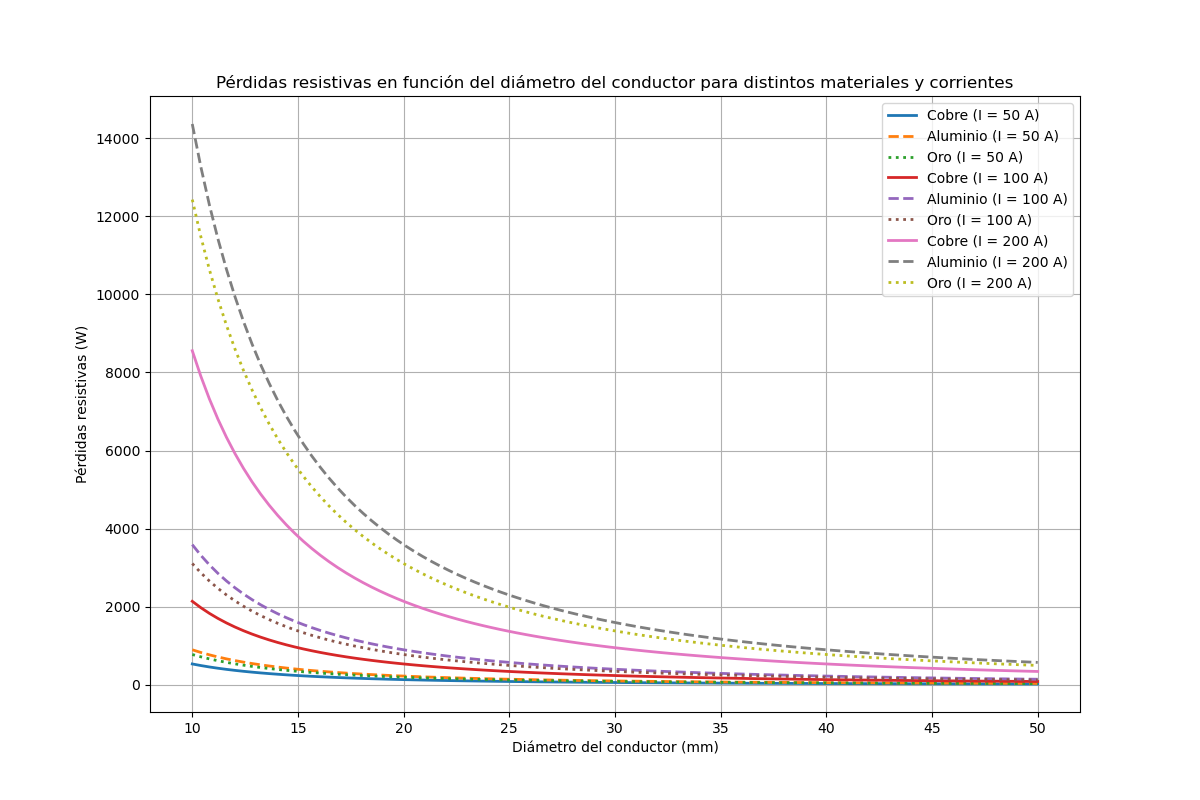
\includegraphics[width=\textwidth]{imagenes/perdidas_resistivas.png}
            \caption{Pérdidas resistivas en función del diámetro del conductor para distintos materiales y corrientes}
            \label{fig:Perdidas_resistivas}
        \end{figure}

       \begin{figure}[H]
           \centering
           \setcounter{figure}{0}
           \renewcommand{\figurename}{Tabla}
           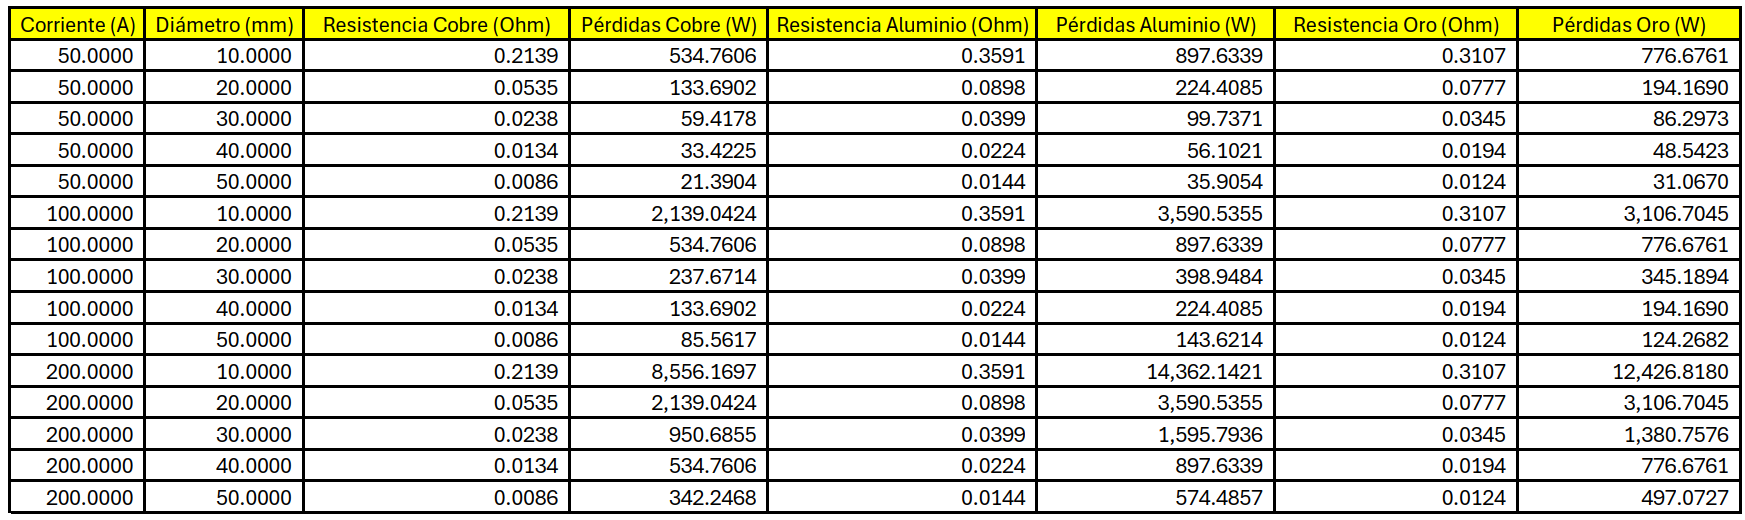
\includegraphics[width=\textwidth]{imagenes/sim_datos_perdidas.png}
           \caption{Tabla de datos de la simulación de Pérdidas resistivas en función del diámetro del conductor para distintos materiales y corrientes}
           \label{fig:sim_datos_perdidas}
       \end{figure}

      Cómo se puede apreciar en la Gráfica \ref{fig:Perdidas_resistivas} y la  Tabla \ref{fig:sim_datos_perdidas}, existe unas diferencias notables, en especial en la Gráfica \ref{fig:Perdidas_resistivas}, evidenciando a simple vista que los diferentes tipos de materiales si son importantes para la mitigación de las pérdidas resistivas del conductor. 

      Por otro lado, los distintos cambios realizado a los parámetros como lo fue la corriente, y su diámetro, trae como consecuencia la acción de aumentar o disminuir las pérdidas; seguidamente sus valores de resistencia, calculado indirectamente debido a los cambios antes efectuado, por ende, se obtuvo una aproximación de ¿Cuál es el material que va a mitigar las perdidas resistivas?

      Como se observa en la figura \ref{fig:awg}, los estándares en calibres van de 0.3606 (mm) a 11.86 (mm), es decir, se hará un énfasis a los valores de la tabla \ref{fig:sim_datos_perdidas}, que serán del 10 (mm) hasta los 30 (mm).

      Con una corriente de $50 \, A$, el cobre obtuvo una disminución con los distintos parámetros, observándose una disminución en sus resistencia y pérdidas, cuando su diámetro aumentaba, al igual que los demás elementos, sin embargo, de estos materiales quien le sigue la menor pérdida sería el oro, por ultimo el aluminio.

      Así mismo, va ocurriendo al aumentar la corriente, demostrando que existe mayor pérdida al tener mas corriente debido al movimiento de carga en el conductor, produciendo en este caso el efecto Joule.

      






\newpage
    
    \section{Conclusiones y posibles aplicaciones}


   En este trabajo se simuló y analizó un caso hipotético en el que se evaluaron las pérdidas resistivas en diferentes conductores, utilizando Python para modelar las propiedades resistivas de cada material. Los conductores analizados fueron cobre, aluminio y oro, considerando distintos valores de resistividad, diámetro y corriente. Esta simulación permitió obtener una visión simplificada de cómo la resistividad y el diámetro del conductor afectan las pérdidas de potencia en una línea de transmisión.

    De acuerdo con los resultados obtenidos, se concluyó que el mejor material para mitigar las pérdidas resistivas en los conductores es el cobre. Si bien el oro también podría ofrecer buenos resultados debido a su baja resistividad, su alto costo y uso limitado en aplicaciones específicas de electrónica lo hacen menos viable para aplicaciones de transmisión a gran escala. Al analizar los datos de la tabla \ref{fig:sim_datos_perdidas}, se observó que las pérdidas con el cobre fueron menores en un $31.15 \%$ en comparación con el aluminio, lo que resulta en una menor resistencia total. Se evidenció que la resistencia es directamente proporcional a las pérdidas resistivas y que estas pueden reducirse aumentando el área transversal del conductor (en este caso, con un cable de longitud fija de 1000 m), ya que un mayor diámetro reduce las pérdidas resistivas.
    
    Por otra parte, tanto el aluminio como el oro pueden descartarse como materiales preferidos para una línea de transmisión, lo que coincide con las prácticas industriales donde el cobre es el material de referencia para la mayoría de los cables conductores, aunque existen excepciones en situaciones específicas.
    
    En cuanto a los métodos de medición de las pérdidas, la elección del procedimiento más adecuado dependerá de las herramientas disponibles, la complejidad del proyecto y la experiencia del personal a cargo. Sin embargo, es importante destacar que las pérdidas en una línea de transmisión pueden medirse de manera simplificada comparando la potencia de entrada con la potencia de salida. Cualquier diferencia entre ambas representaría la cantidad de energía disipada en forma de calor debido a las pérdidas resistivas.
    
    Finalmente, en la sección \ref{sec:dispositivos} se presentaron distintos dispositivos y técnicas para mitigar las pérdidas en sistemas eléctricos, proporcionando alternativas para mejorar la eficiencia. Aunque inicialmente se consideró la posibilidad de simular los circuitos mediante herramientas como Multisim, Proteus o LTSpice, se optó por un enfoque más eficiente y directo, centrado en la simulación de las pérdidas resistivas en los conductores, lo que permitió demostrar con claridad los efectos de la resistividad y el diámetro en la eficiencia del sistema.


\newpage

    
    \printbibliography

    %\nocite{*}
    
\label{Lastpage}

\end{document}

